% !TEX root = ../thesis.tex

\chapter{Results}
\label{ch:results}

% Research-question driven structure: after a short preliminary that fixes
% the representative HealthGAN sample, each top-level section directly
% answers one of the three research questions stated in
% §\ref{sec:intro:rqs}. All numerical findings live in this chapter; metric
% definitions remain in Section~\ref{sec:method:evaluation}.


\section{RQ1 - Methods and Metrics for Evaluating Synthetic Medical Data}
\label{sec:results:rq1}

% RQ1 asks which methods and metrics are suitable for evaluating the utility
% and privacy risk of synthetic tabular medical data, and what distinct
% dimension each captures. This section answers that question before the
% generator rankings of RQ2 and RQ3.

\subsection{Full Evaluation Framework}
\label{sec:results:rq1:operationalising}

RQ1 is evaluated by several groups of complementary metrics rather 
than a single score. At the top level, the thesis separates \emph{utility} from
\emph{privacy}. Utility is divided into statistical similarity and
predictive performance, because a synthetic table can reproduce marginal
distributions while still failing as training data for a downstream
model. Privacy is evaluated separately through distance-based, inference-based,
and outlier/linkability analyses. The full operational definitions are given in
Section~\ref{sec:method:evaluation}. This section explains why the
components are jointly necessary for answering RQ1.

The full protocol contains both headline single-number metrics and
supporting evaluations. The headline metrics are used in the comprehensive
summary table and aggregate views. The supporting evaluations
are kept because they explain why a headline metric changes and expose
failure modes that a scalar can hide.

The summary in Table~\ref{tab:rq2:summary} reports the
twelve main metrics selected from the evaluation measures listed in
Table~\ref{tab:rq1-coverage}. It is a
compact scalar subset of that framework, not a separate set of metrics.
The evaluation measures not included in the summary can be divided into
two groups. The first is inherently visual and has no single value to tabulate. 
The second is scalar but already covered by a stronger
summary on the same axis. For example, the mean and standard-deviation checks are
subsumed by the more shape-sensitive mean KS. NNAA
measures nearest-neighbour train-test resemblance, whereas membership
inference measures attack-based train/non-member distinguishability.
Including both measures in the main summary shows that two separate
memorisation tests indicate similarly negligible privacy concern.

\subsection{Metric Coverage and Blind Spots}
\label{sec:results:rq1:diagnostic}

Table~\ref{tab:rq1-coverage} summarises the distinct role of each metric
family in the framework. The table is deliberately organised by
measurement role rather than by generator result. Its purpose is to 
show that the evaluation measures provide
complementary information. Each captures one aspect of
synthetic-data quality and leaves a blind spot that motivates reporting it
alongside the others.

\begin{table}[!htbp]
\centering
\footnotesize
\setlength{\tabcolsep}{3.5pt}
\caption{Coverage of the evaluation framework for RQ1. Each instrument
captures a different utility or privacy dimension and has a blind spot
significant that requires complementary metrics or diagnostics.}
\label{tab:rq1-coverage}
\begin{tabular}{p{2.0cm}p{3.2cm}p{4.0cm}p{4.2cm}}
\toprule
Branch & Instrument & Captured dimension & Main blind spot or role \\
\midrule
Similarity & Marginal plots and mean and standard-deviation checks & Column-level distribution, scale, and support failures & Descriptive and visual; does not summarise joint structure \\
Similarity & Mean Kolmogorov-Smirnov statistic & Worst-case marginal distribution discrepancy averaged across columns & Column-wise only; cannot detect dependency errors \\
Similarity & Pairwise correlation difference and heatmaps & Preservation of joint linear dependency structure & Blind to non-linear and higher-order interactions \\
Similarity & PCA visual projection & Overlap in the first two principal components & Encoding-dependent two-dimensional linear projection; overlap does not establish distributional fidelity \\
\midrule
Predictive & TSTR AUC-ROC, F1, precision, recall, and ROC curves & Transferability of conditional structure to downstream classifiers & Depends on classifier choice and threshold; does not test clinical effect sizes \\
Predictive & Feature-importance agreement & Whether synthetic-trained models rely on similar predictors & Model-specific interpretability diagnostic rather than a clinical truth claim \\
Predictive & Cox confidence interval overlap & Agreement of clinically interpretable hazard-ratio estimates & Coarser than classifier metrics and tied to the Cox model specification \\
\midrule
Privacy & Nearest-neighbour distance and NNDR & Raw and scale-normalised proximity of synthetic records to real records & High distance can reflect off-manifold collapse rather than protection \\
Privacy & NNAA and privacy loss & Real-synthetic distinguishability and train-test memorisation gap & Covers only the memorisation axis; blind to conditional attribute leakage and outlier/tail disclosure \\
Privacy & Membership-inference advantage & Training-set membership leakage under a distance-based adversary & Does not test conditional leakage of specific sensitive attributes \\
Privacy & Attribute-inference advantage & Conditional leakage of selected sensitive attributes & Limited to the selected attributes and attacker design \\
Privacy & Outlier linkability & Tail-record disclosure risk for rare or extreme records & Depends on the outlier definition and neighbourhood radius \\
\midrule
Aggregation & Table, landscape, radar, and heatmap & Communication of trade-offs across utility and privacy dimensions & Interpretive only; raw metric values remain the evidential basis \\
\bottomrule
\end{tabular}
\end{table}

The framework therefore contains deliberate overlap, but not unnecessary
duplication. For example, AUC-ROC and F1 both evaluate downstream
classification, but they answer different questions. AUC-ROC measures
threshold-independent ranking quality, while F1 exposes behaviour at the
chosen decision threshold. Likewise, nearest-neighbour distance and NNDR
both measure proximity, but NNDR makes that proximity interpretable
relative to the real data's own spacing. Membership-inference AUC and
membership-inference advantage report the same attack on two scales. 
The advantage measure is retained because it directly shows how much the
attack outperforms random guessing.

\subsection{Empirical Usefulness on the Benchmark}
\label{sec:results:rq1:empirical}

The empirical results in Section~\ref{sec:results:rq2} show that the
metrics were not equally discriminative. The strongest separation came
from the marginal and joint similarity metrics like TSTR AUC-ROC,
nearest-neighbour distance ratio, attribute-inference and outlier
linkability audits. Mean KS, PCD, and PCA projection separated the
off-manifold PATE-GAN output from the other four generators, while PCD
also distinguished the stronger joint-structure preservation of
Pythia-1B. TSTR AUC-ROC provided the clearest predictive-utility ordering
across all five generators and made the LLM-side differential-privacy cost
visible.

Several diagnostics were less decisive for ranking but important for
interpretation. Per-column plots showed the specific distributional failures underlying
PATE-GAN's poor scalar similarity scores. The ROC curves showed that the AUC ranking 
remained consistent across different classification thresholds. Feature-importance and Cox
agreement checked whether predictive utility was supported by comparable
predictor structure and clinically interpretable effect estimates.
Membership inference and NNAA privacy loss were nearly flat across
generators, but they are still useful safeguards. Their near-zero values
support the conclusion that the observed privacy differences are not driven
by direct training-set memorisation. On the other hand, attribute inference
identified the clearest privacy benefit of the differentially private LLM
variant, since it removed the mild primary-diagnosis leakage observed for
Pythia-1B.

\subsection{Recommended Minimal Evaluation Suite}
\label{sec:results:rq1:minimal-suite}

The minimal suite is not intended to replace the full evaluation protocol
used in this thesis. The full protocol remains necessary for validation,
interpretation, and sensitivity checks. The minimal suite is instead a
practical recommendation for future studies that need a compact first-pass
evaluation while still covering the main utility and privacy failure
modes.

For such a compact evaluation, the recommended core metrics are:
mean KS, pairwise correlation difference, TSTR AUC-ROC, median NNDR,
membership-inference advantage, maximum attribute-inference advantage, and
outlier linkability. Mean KS measures marginal fidelity, while PCD measures the preservation
of pairwise linear relationships. TSTR AUC-ROC evaluates downstream
predictive utility, and median NNDR measures scale-normalised record
proximity. Membership-inference advantage assesses overall training-set
leakage, attribute-inference advantage evaluates sensitive-attribute
leakage, and outlier linkability measures the disclosure risk of rare
records. In medical applications where interpretable
effect preservation is central, Cox confidence-interval overlap should be
added to this minimal suite. Feature-importance agreement should also be retained
where model interpretability is important.

\subsection*{Findings for Research Question 1}
\label{sec:results:rq1:answer}

RQ1 is answered by a two-pillar evaluation framework rather than by a
single metric. Utility requires separate assessment of marginal
fidelity, pairwise linear-dependency fidelity and downstream predictive
performance. Preservation of clinically interpretable association
should also be considered where applicable. 
Privacy should not be limited to one measure. It should be
examined through record proximity, membership-inference, attribute
inference, and outlier-specific linkability. Aggregate views can
communicate the resulting profiles, but they remain interpretive
summaries rather than replacements for the raw metric values.

The recommended metrics cover non-equivalent failure modes. 
Mean KS measures marginal distribution fidelity, pairwise 
correlation difference measures preservation of linear 
dependencies, and TSTR AUC-ROC evaluates the transfer of predictive 
structure. The privacy metrics examine different forms of disclosure risk. Median
NNDR measures how close synthetic records are to real records relative to
the spacing within the real data. Membership-inference advantage measures
the risk of identifying training records. Maximum attribute-inference
advantage measures leakage of sensitive attributes. Outlier linkability
evaluates disclosure risk for rare records. When several 
metrics evaluate the same aspect, the compact suite retains
the more informative summary. Mean KS is used instead of moment checks,
and NNDR is used instead of raw nearest-neighbour distance. 
Membership-inference advantage is reported because it directly shows how
much the attack performs above or below random guessing. TSTR AUC-ROC is used as the main
threshold-independent measure of predictive performance. The omitted 
measures nevertheless remain useful as supporting evaluation 
or application-specific checks.

The results show that these metrics did not differentiate 
the generators equally well. Mean KS, pairwise correlation difference, and TSTR
AUC-ROC provided the clearest utility-side separation. Membership
inference and NNAA privacy loss remained close to their reference values
across generators, while outlier linkability was consistently low.
Among the usable generators, median NNDR distinguished HealthGAN's 
record spacing from that of the LLM-based generators. Maximum 
attribute-inference advantage detected the primary-diagnosis leakage 
observed for Pythia-1B but not for Pythia-1B-DP. 
The limited empirical separation provided by membership-inference 
advantage and outlier linkability does not make them redundant. 
They are retained because they audit distinct disclosure risks, 
and their near-reference values document the absence of observed 
leakage under those tests. PATE-GAN provided 
the clearest demonstration of metric complementarity. It has the large 
nearest-neighbour distances and zero outlier linkability occurred 
alongside poor statistical similarity and predictive utility. 
Distance-based privacy results must therefore be
interpreted together with fidelity and attack-based diagnostics.

For compact first-pass evaluation, the seven-metric core defined in
Section~\ref{sec:results:rq1:minimal-suite} covers the general utility
and privacy dimensions. Cox confidence-interval overlap should be added
when preservation of clinically interpretable associations is relevant
to the intended use, while feature-importance agreement should be
retained when predictor interpretation is required. This reduced suite
supports initial screening but does not replace the complete evaluation
protocol.


\section{RQ2 - The Privacy-Utility Landscape Across Five Generators}
\label{sec:results:rq2}

% RQ2 (finalised): "How do GAN-based and LLM-based synthesisers compare on
% the privacy-utility trade-off when applied to tabular medical data, and
% which achieves a more effective balance?"
%
% Scope: five generators are positioned on a single privacy-utility plane
%  (HealthGAN, PATE-GAN, Pythia-70M, Pythia-1B, Pythia-1B-DP). PATE-GAN
% appears here for landscape completeness despite incorporating DP by
% construction; this is acknowledged in the figure caption and discussed
% further in \S\ref{sec:discussion:limit:pategan-dual-role}. The
% within-family DP-toggle analysis (HealthGAN $\to$ PATE-GAN; Pythia-1B
% $\to$ Pythia-1B-DP) is reported separately in \S\ref{sec:results:rq3}.

\subsection{Utility Results}
\label{sec:results:rq2:utility}

This subsection assesses how each generator preserves the
analytical value of the real data, reported through two complementary
blocks. The first, statistical similarity
(Section~\ref{sec:results:rq2:utility:similarity}), examines how closely
the synthetic distributions reproduce the marginal, pairwise, and joint
structure of the reference data. The second, predictive performance
(Section~\ref{sec:results:rq2:utility:predictive}), quantifies the extent
to which models trained on synthetic data retain their accuracy when
evaluated on real records, thereby capturing utility for downstream
machine-learning tasks.

% Utility is reported in two complementary blocks: statistical similarity
% (Section~\ref{sec:eval:utility:similarity}, notebook cells 29–34) and
% predictive performance (Section~\ref{sec:eval:utility:predictive}, cells
% 35–41).

\subsubsection{Statistical Similarity}
\label{sec:results:rq2:utility:similarity}

Statistical similarity is reported along the three complementary views
defined in Section~\ref{sec:eval:utility:similarity}: per-column marginal
agreement, pairwise linear-dependency agreement, and two-dimensional PCA visualisation. 
All five generators and the real reference are
evaluated on the aligned feature space introduced in
Section~\ref{sec:data:fe}.

\paragraph{Per-Column Marginal Distributions:}
Figure~\ref{fig:rq2:marginals}  compares the real and synthetic marginals
for a representative block of columns spanning ordinal field
(\emph{age}), binary outcome (\emph{readmitted}), categorical codes
(\emph{admission\_\allowbreak type\_\allowbreak id}, \emph{A1Cresult}). 
Figure~\ref{fig:rq2:marginals-continuous} presents the continuous clinical
counts (\emph{time\_\allowbreak in\_\allowbreak hospital},
\emph{num\_\allowbreak lab\_\allowbreak procedures},
\emph{num\_\allowbreak medications},
\emph{number\_\allowbreak inpatient}). 

\begin{figure}[H]
\centering
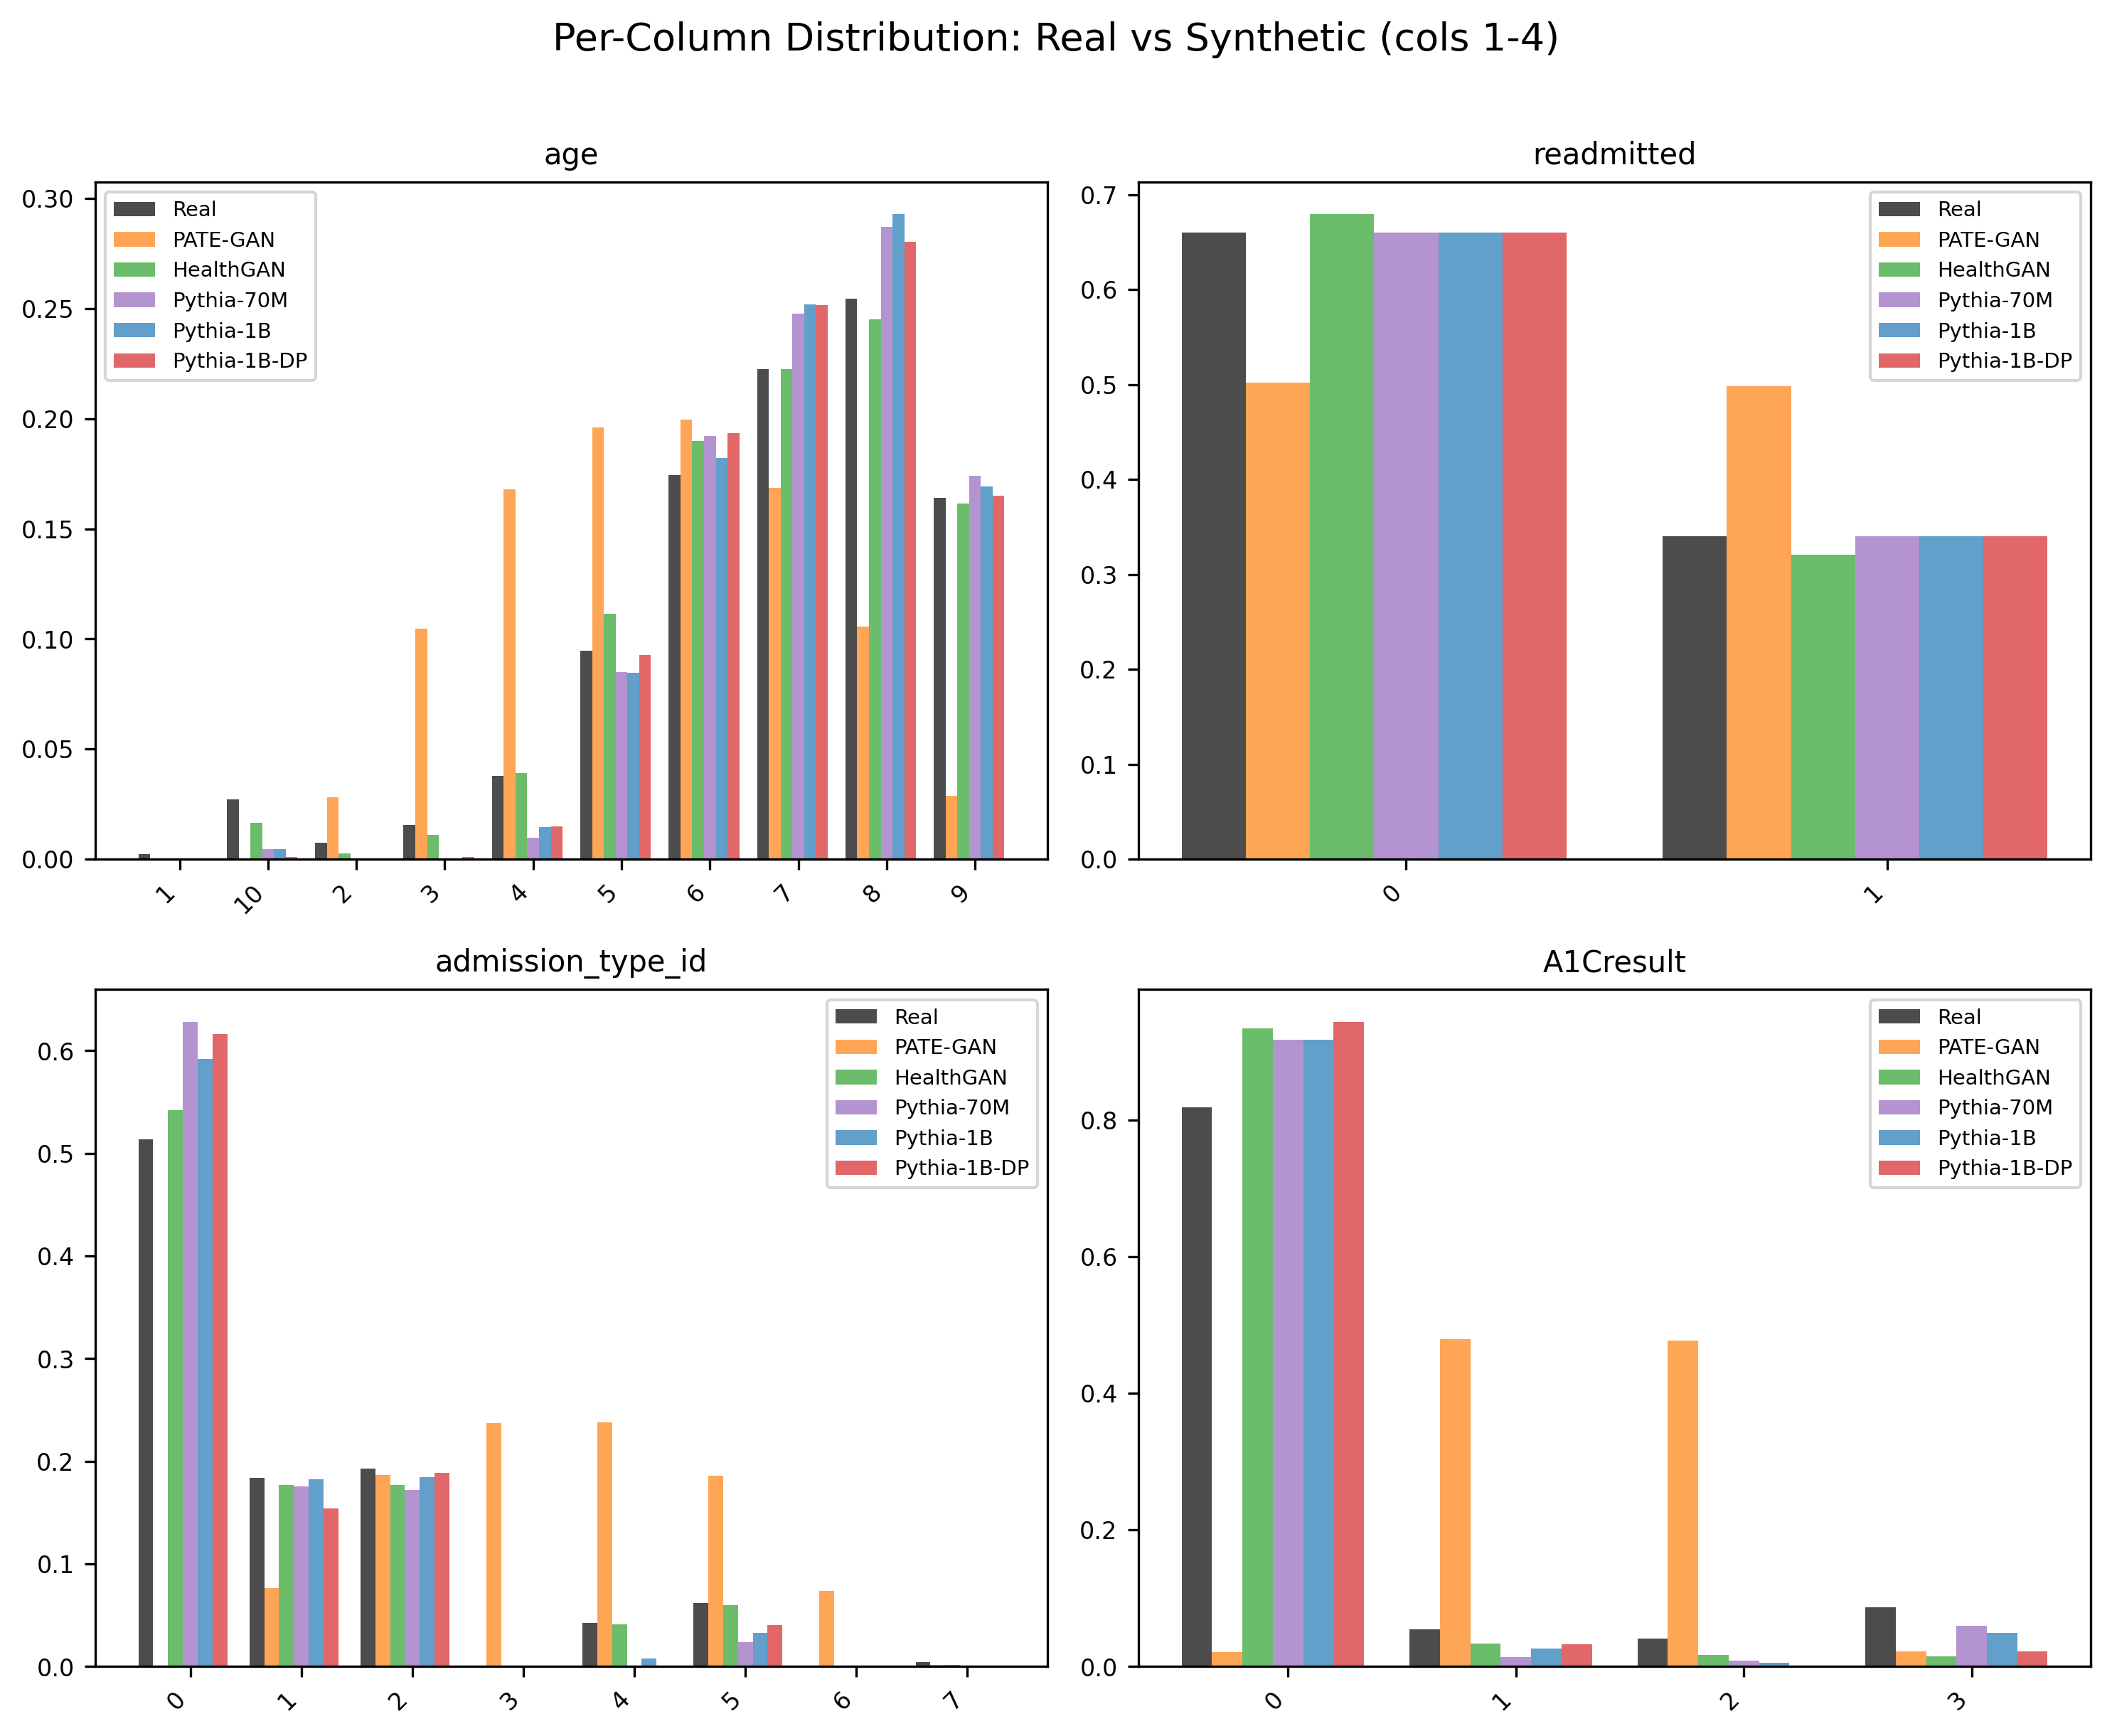
\includegraphics[width=0.90\textwidth]
{images/results/1a-per_column_distribution_reordered_1}
\caption{Representative marginal distributions for ordinal, binary, and
categorical columns, comparing the real data with five synthetic
generators. HealthGAN and the three Pythia variants closely match the real
reference, while PATE-GAN distorts the categorical marginals.}
\label{fig:rq2:marginals}
\end{figure}

\begin{figure}[H]
\centering
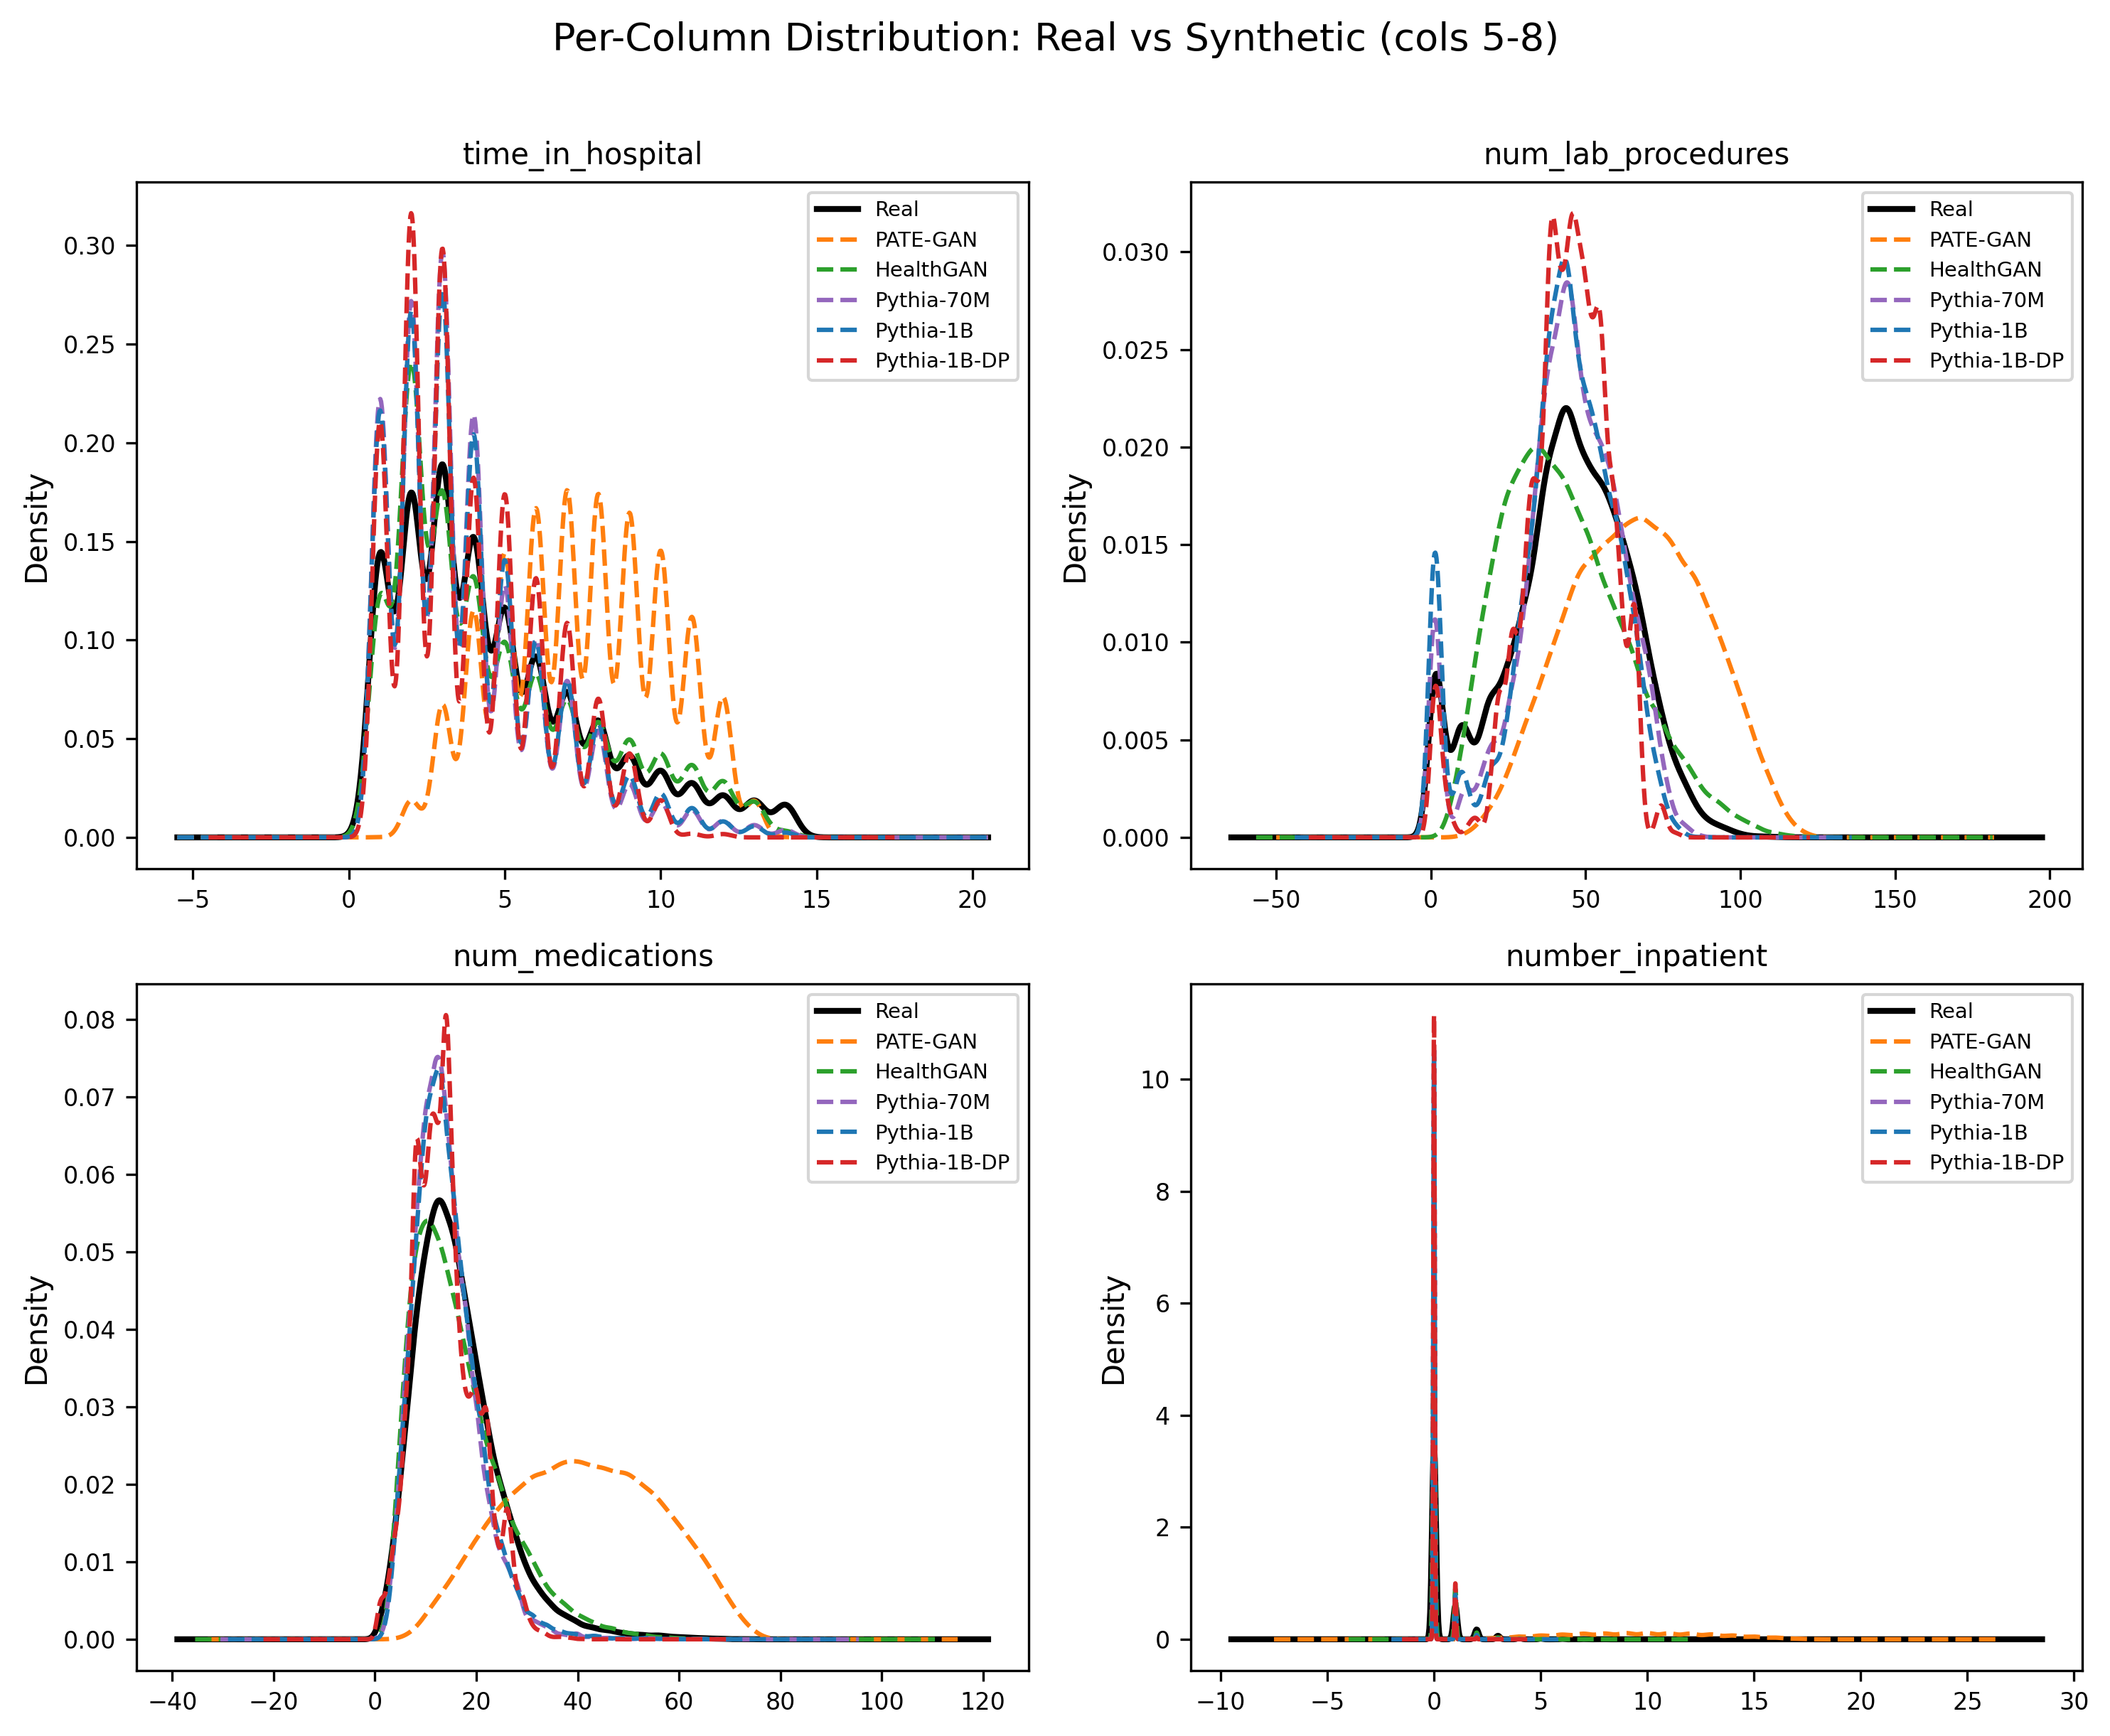
\includegraphics[width=0.90\textwidth]
{images/results/1a-per_column_distribution_reordered_2}
\caption{Representative marginal distributions for continuous
clinical-count columns, comparing the real data with five synthetic
generators. HealthGAN and the three Pythia variants closely match the real
reference, while PATE-GAN distorts the continuous marginals.}
\label{fig:rq2:marginals-continuous}
\end{figure}

Four of the five
generators, namely HealthGAN and the three Pythia variants, reproduce the
real marginals closely. Their bar charts and density curves closely match 
the real reference data for both categorical and continuous variables. 
PATE-GAN is the consistent
exception. It flattens the \emph{readmitted} distribution towards an even
split rather than the real 66:34 ratio, assigns substantial probability
mass to \emph{age} and \emph{admission\_\allowbreak type\_\allowbreak id} categories that are
rare or absent in the real data. From the other columns, we can also see that PATE-GAN's
distribution is placed mostly on either dominant categories or for continuous colmns they
are mostly smooth distribution near the median. This is the earilest sign that PATE-GAN 
is not learning the read data distribution well and is instead producing a distorted output.
The full per-column gallery for all five generators is provided in Appendix~\ref{app:distributions}.


\paragraph{Marginal and Joint Similarity Scores:}
Table~\ref{tab:rq2:ks-pcd} reduces the per-column comparison to two
headline scalars defined in
Sections~\ref{sec:eval:utility:similarity:ks}
and~\ref{sec:eval:utility:similarity:pcd}: i) mean Kolmogorov-Smirnov
(KS) statistic averaged across columns, which averages each
column's largest empirical-distribution difference, and ii) mean pairwise correlation difference (PCD),
which measures the fidelity of the joint linear-dependency structure.
The full per-column KS values behind the mean are
tabulated in Appendix~\ref{app:ks-per-column}.

Throughout the result tables, $\uparrow$ indicates that higher values are
preferable, whereas $\downarrow$ indicates that lower values are preferable.
For tables reporting $\Delta$, the sign should therefore be interpreted
relative to this direction. A positive change is favourable for $\uparrow$
metrics but unfavourable for $\downarrow$ metrics.

\begin{table}[!htbp]
\centering
\small
\caption{Mean Kolmogorov-Smirnov statistic and mean pairwise correlation
difference per generator (lower is better on both). KS is averaged over
all compared columns, PCD is the mean absolute difference between the real
and synthetic correlation matrices. The best non-trivial value in each
column is shown in bold.}
\label{tab:rq2:ks-pcd}
% Auto-generated by data_analysis.ipynb (1d). Do not edit by hand.
% Requires booktabs.
\begin{tabular}{lcc}
\toprule
Generator & Mean KS $\downarrow$ & PCD $\downarrow$ \\
\midrule
PATE-GAN & 0.5381 & 0.1142 \\
HealthGAN & \textbf{0.0480} & 0.0336 \\
Pythia-70M & 0.0856 & 0.0308 \\
Pythia-1B & 0.0805 & \textbf{0.0206} \\
Pythia-1B-DP & 0.0992 & 0.0466 \\
\bottomrule
\end{tabular}

\end{table}

The two scalars confirm the visual reading. HealthGAN attains the lowest
mean KS and Pythia-1B the lowest PCD, with the four non-PATE generators all falling
in a narrow band (mean KS $0.048$-$0.099$; PCD $0.021$-$0.047$).
PATE-GAN is more than an order of magnitude worse on the marginal axis
(mean KS $0.5381$) and three to five times worse on the joint axis
(PCD $0.1142$). Thus places it in a separate regime from every other
generator. Within the LLM family, the differentially private variant is
modestly worse than its non-private counterpart on both axes (mean KS
$0.0992$ vs.\ $0.0805$; PCD $0.0466$ vs.\ $0.0206$). it is an early indication
of the differential-privacy utility cost quantified within-family in
Section~\ref{sec:results:rq3:llm-toggle}.

\paragraph{Correlation Structure:}
Figure~\ref{fig:rq2:corrheat} contrasts the correlation-difference
heatmaps (real minus synthetic correlation matrix) of the two
joint-similarity extremes. PATE-GAN exhibits dense blocks of large
residual correlation across the clinical and medication columns,
indicating that the dependency structure of its output departs
substantially from the real data. Pythia-1B is near-uniformly pale,
indicating that most pairwise correlations are reproduced to within a
small residual. The corresponding heatmaps for the remaining three
generators (HealthGAN, Pythia-70M, and Pythia-1B-DP), consistent with
the PCD ordering of Table~\ref{tab:rq2:ks-pcd}, are collected in
Appendix~\ref{app:corrheat}.

\begin{table}[H]
\centering
\caption{Mean Absolute Correlation Difference across models.}
\label{tab:mean-absolute-correlation-difference}
\begin{tabular}{lc}
\hline
\textbf{Model} & \textbf{Mean Absolute Correlation Difference} \\
\hline
PATE-GAN      & 0.1142 \\
HealthGAN     & 0.0336 \\
Pythia-70M    & 0.0308 \\
Pythia-1B     & \textbf{0.0206} \\
Pythia-1B-DP  & 0.0466 \\
\hline
\end{tabular}
\end{table}

The quantitative results are consistent with the patterns observed in the
correlation-difference heatmaps. Pythia-1B achieves the lowest mean
absolute correlation difference (0.0206), indicating the closest
reproduction of the real data's correlation structure, whereas
PATE-GAN records the highest difference (0.1142). HealthGAN and
Pythia-70M perform comparably, while the higher value of Pythia-1B-DP
suggests that differential privacy reduces correlation fidelity.

\begin{figure}[H]
\centering

\begin{subfigure}{\textwidth}
\centering
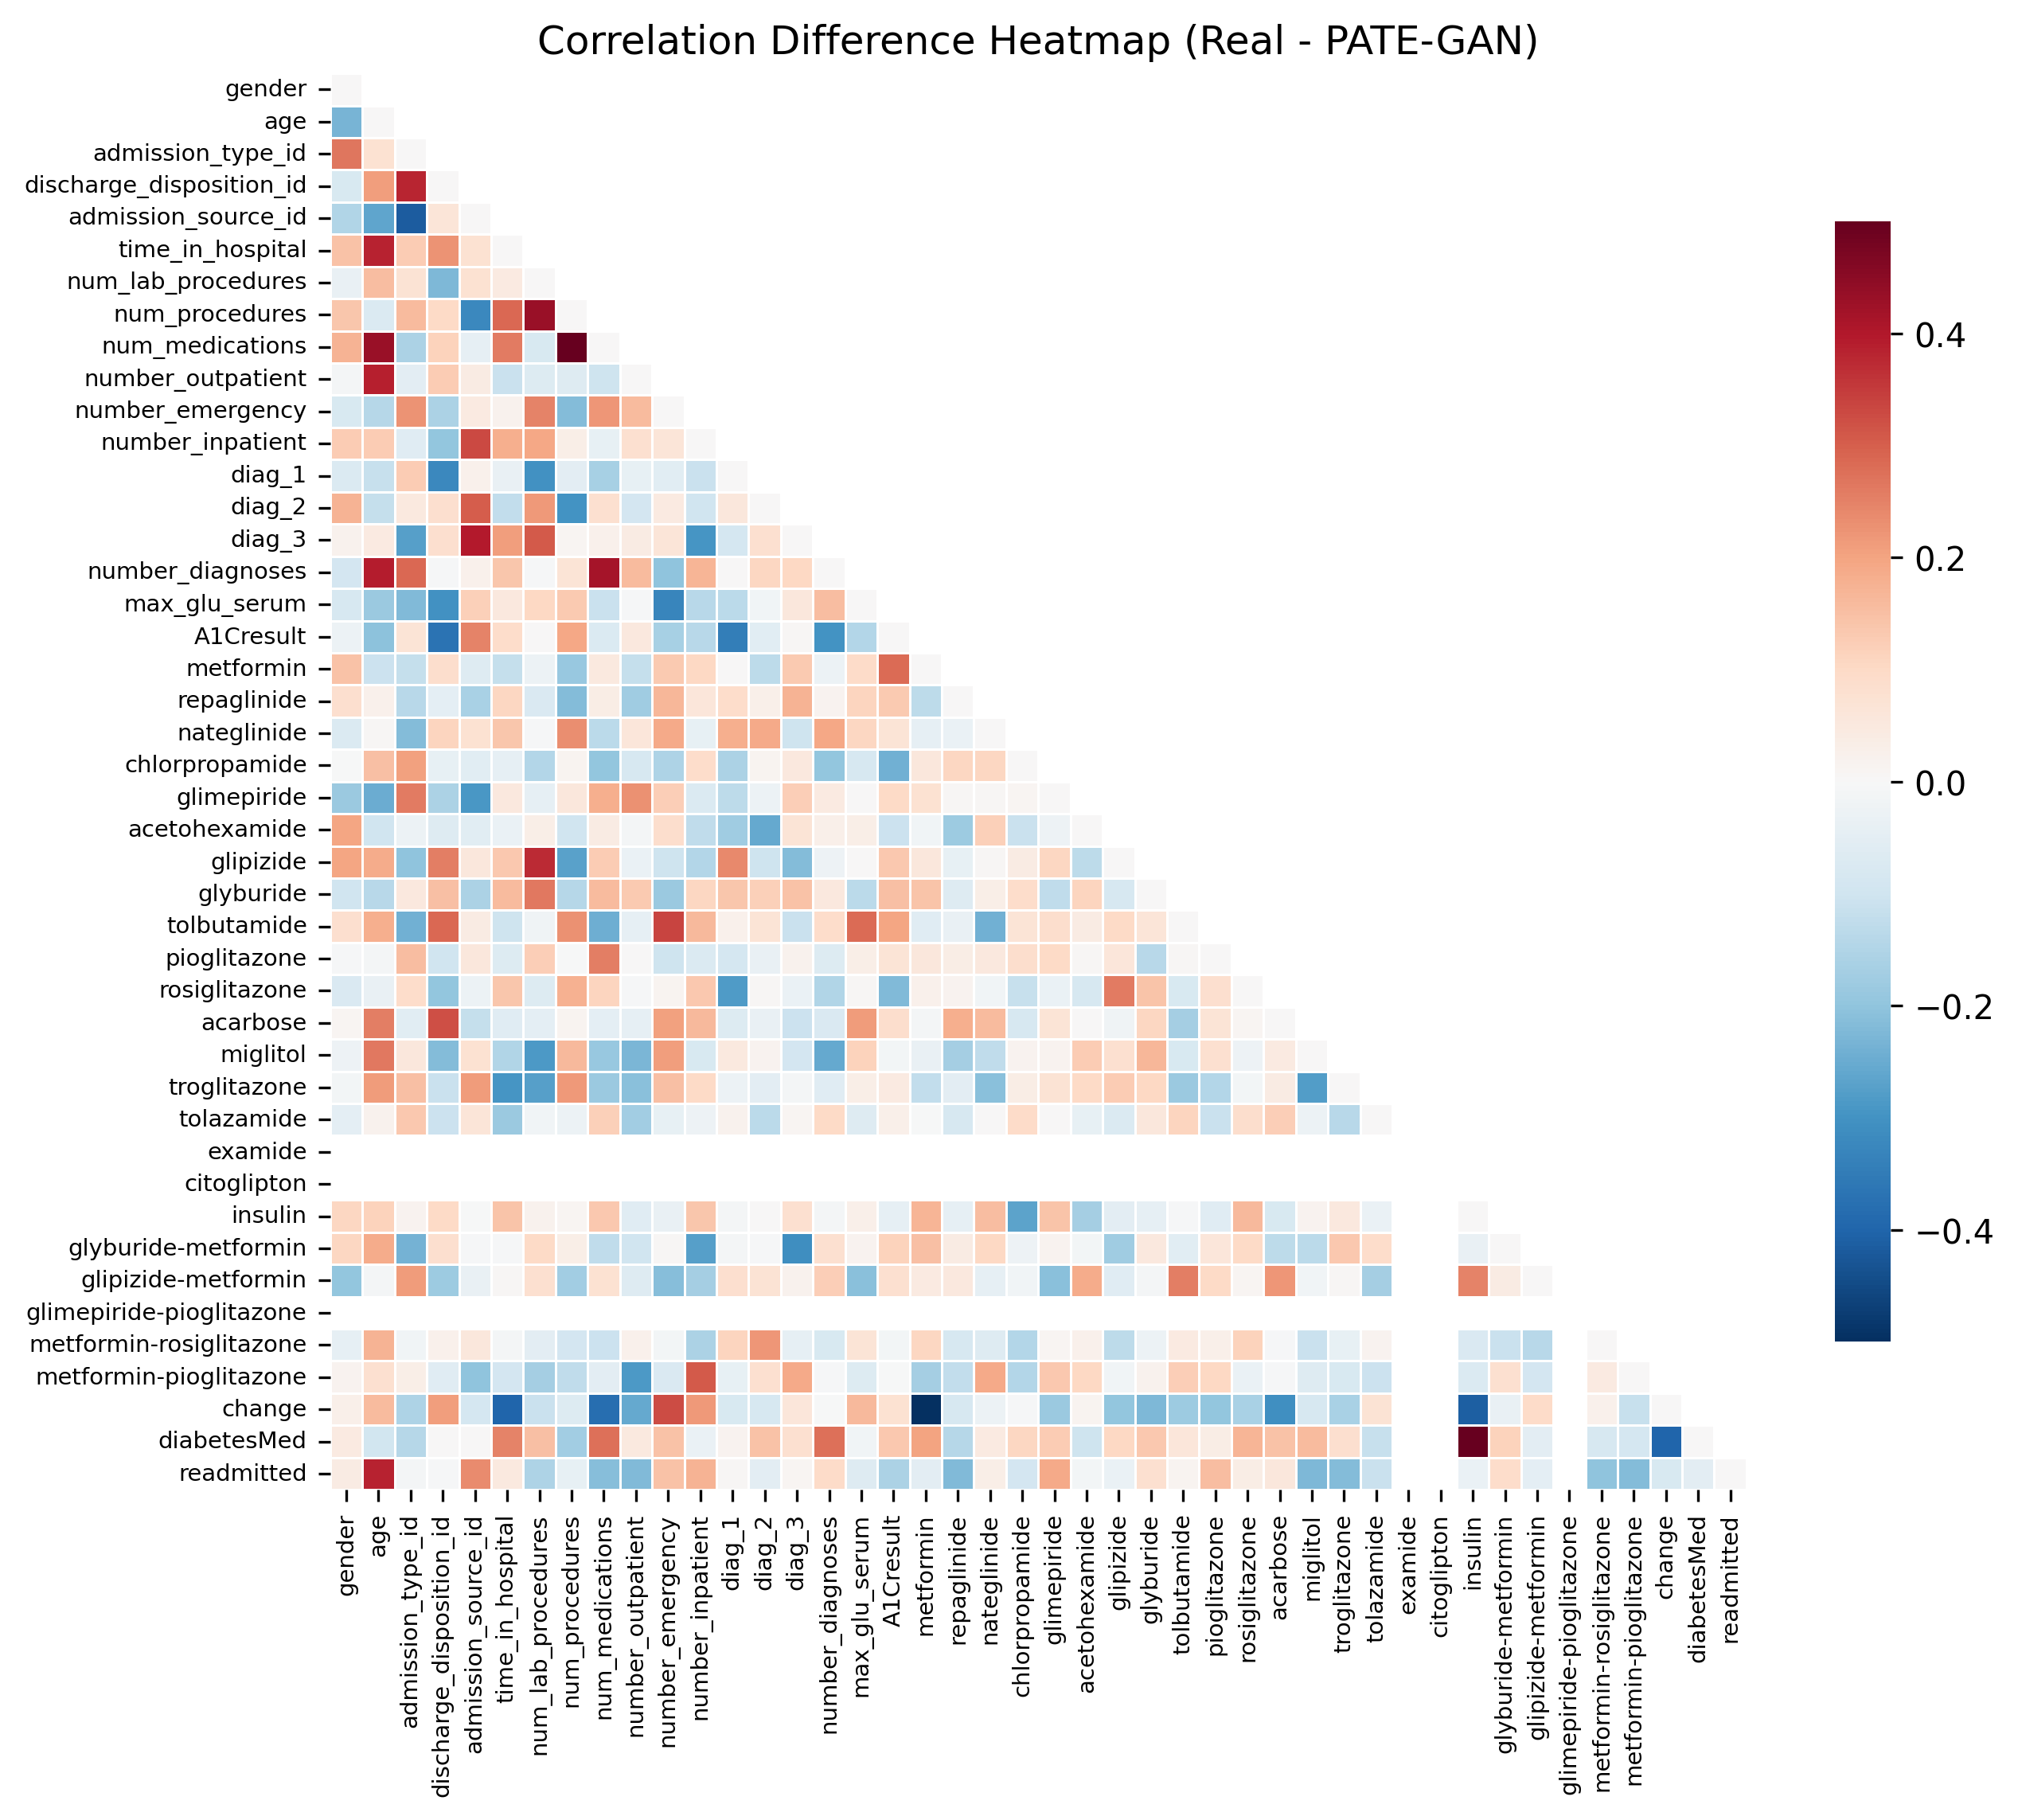
\includegraphics[
    width=\textwidth,
    height=0.45\textheight,
    keepaspectratio
]{images/results/1c-corr_diff_heatmap_1}
\caption{PATE-GAN.}
\end{subfigure}

\vspace{1em}

\begin{subfigure}{\textwidth}
\centering
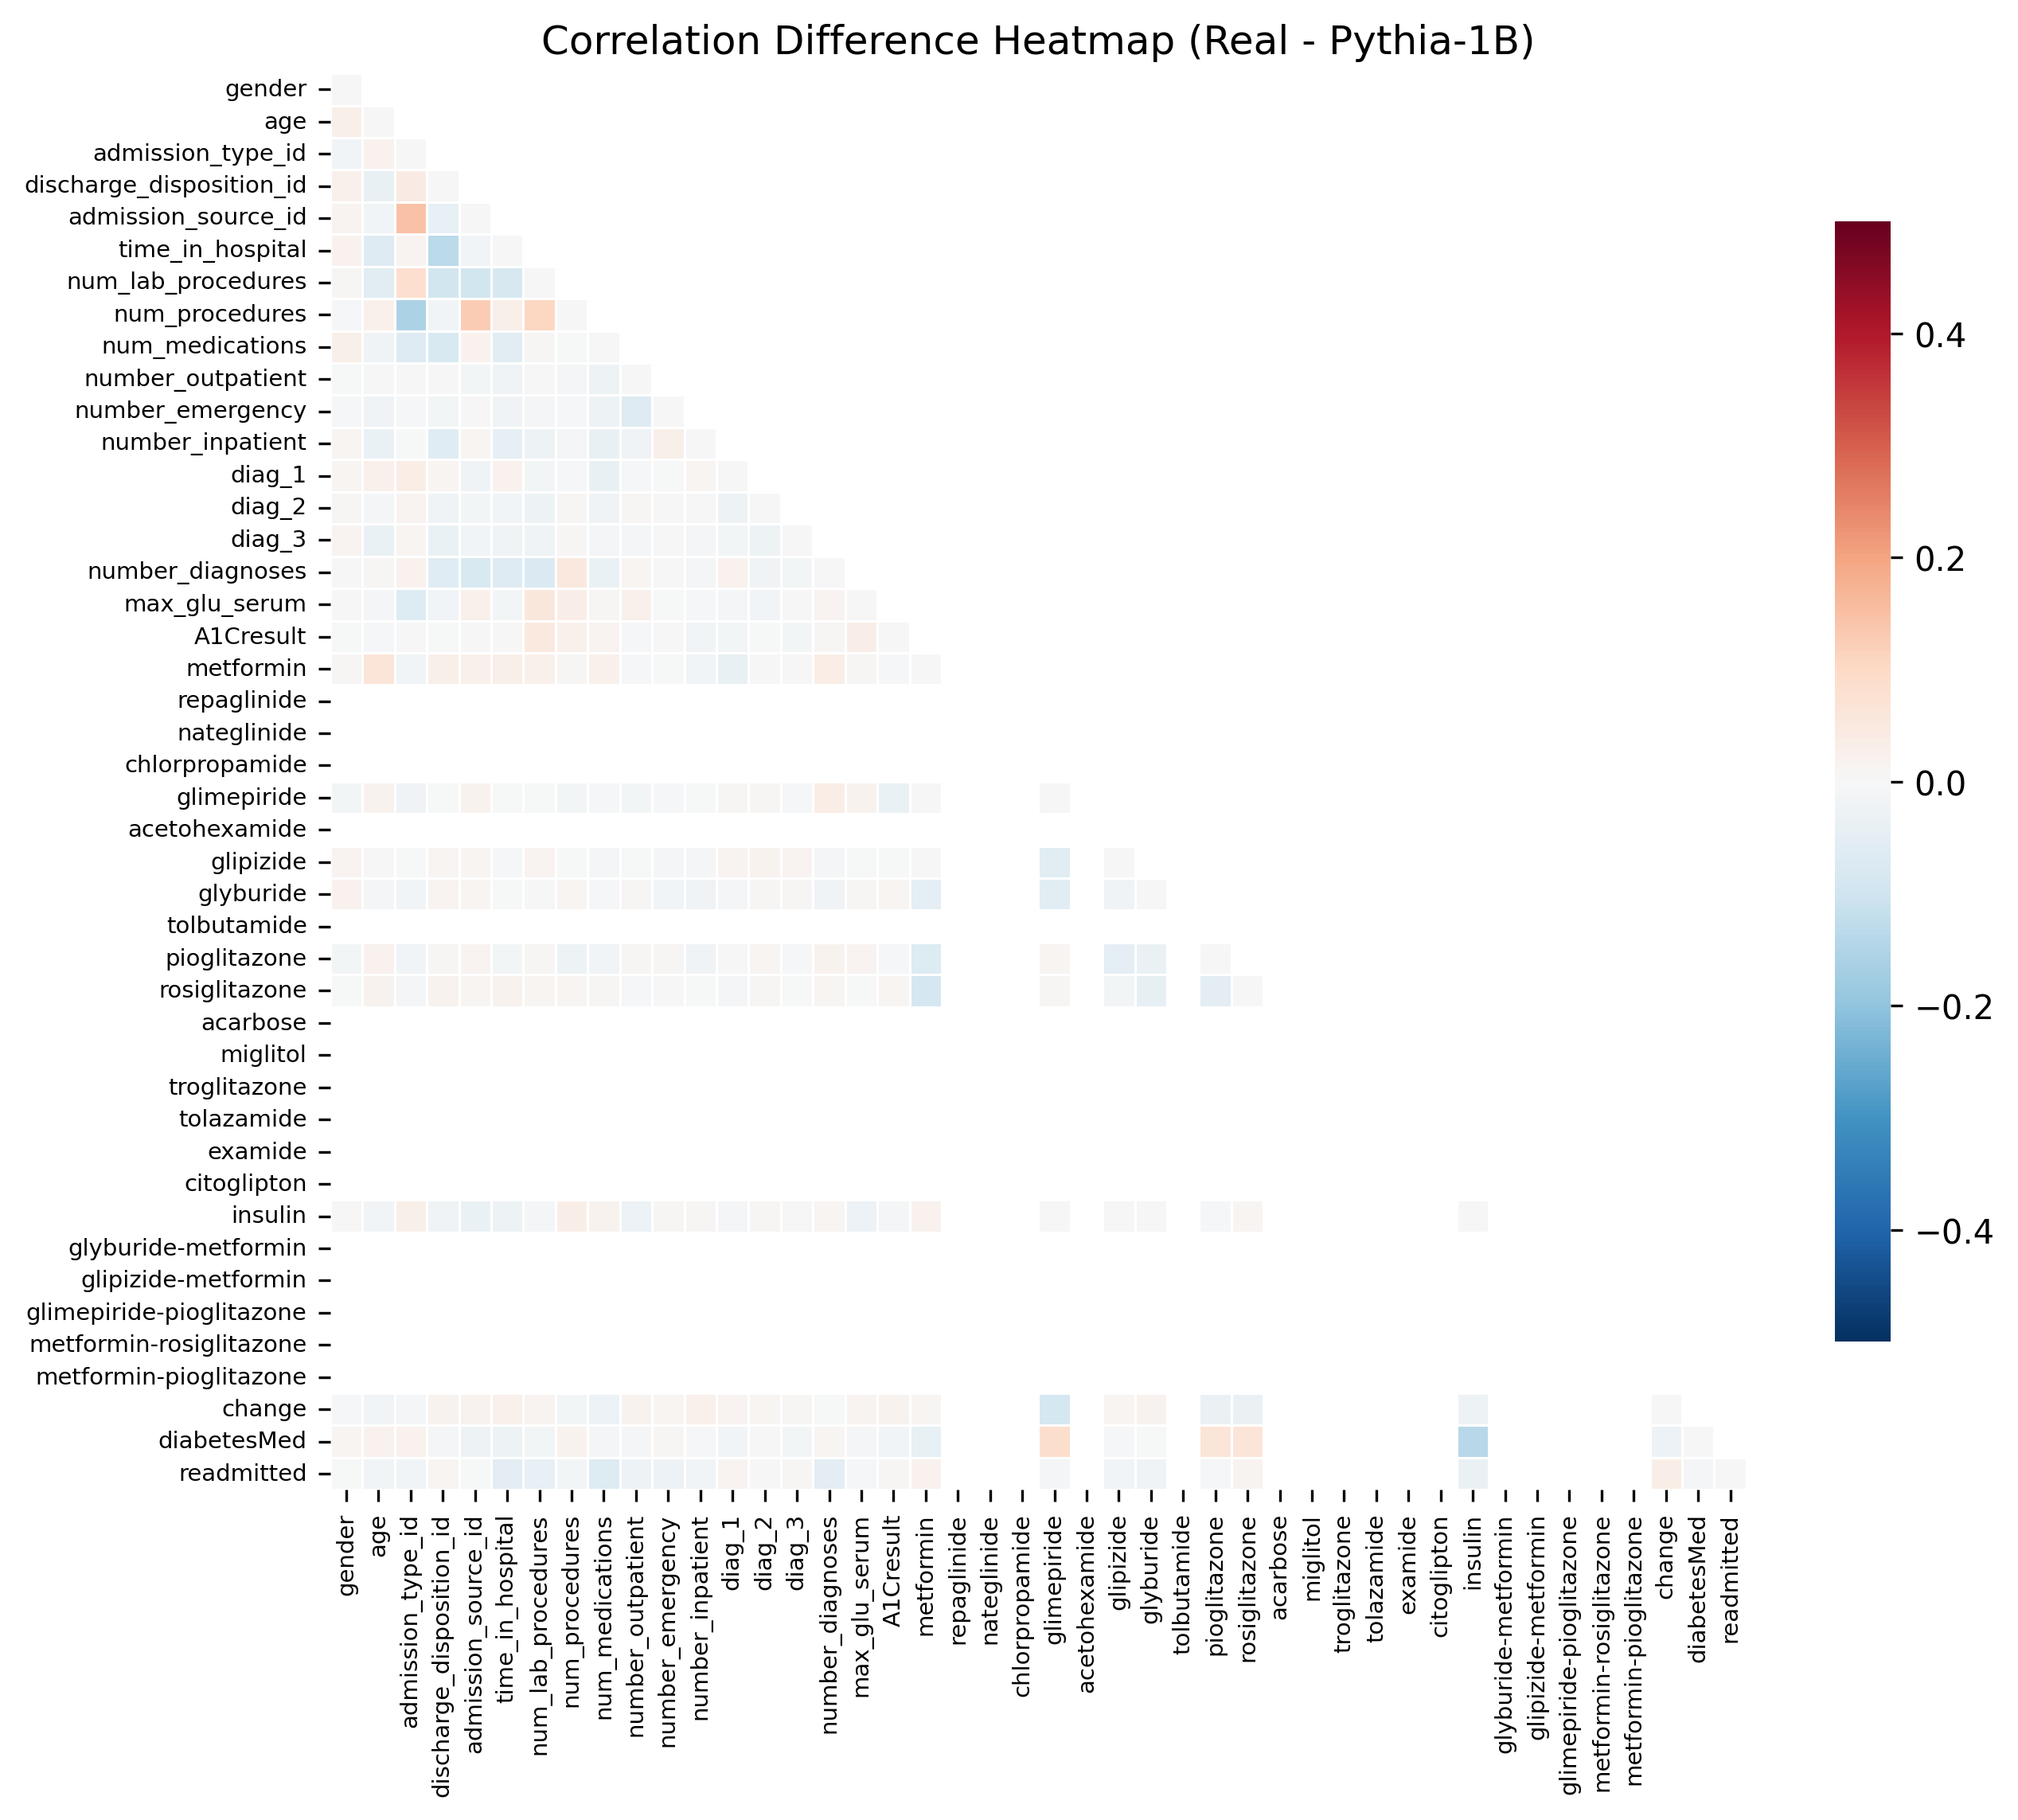
\includegraphics[
    width=\textwidth,
    height=0.45\textheight,
    keepaspectratio
]{images/results/1c-corr_diff_heatmap_4}
\caption{Pythia-1B.}
\end{subfigure}

\caption{Correlation-difference heatmaps comparing the real and synthetic
correlation matrices. PATE-GAN shows large residual correlations, while
Pythia-1B more closely reproduces the real correlation structure.}
\label{fig:rq2:corrheat}
\end{figure}

\paragraph{PCA-Based Manifold Overlap:}
Figure~\ref{fig:rq2:pca} projects the real and synthetic records onto the
first two principal components estimated from the combined real-plus-synthetic table
(Section~\ref{sec:eval:utility:similarity:pca}). The real cloud and four
of the five synthetic clouds occupy a common region of the projected
space, whereas PATE-GAN forms a disjoint cluster displaced along the
first principal component. The projection therefore represents at the
joint level what the marginal and correlation views establish separately.
PATE-GAN’s samples differ from the real-data distribution, 
while those of the other four generators align closely with it. This also 
aligns with our previous observation of PATE-GAN.
\begin{figure}[H]
\centering
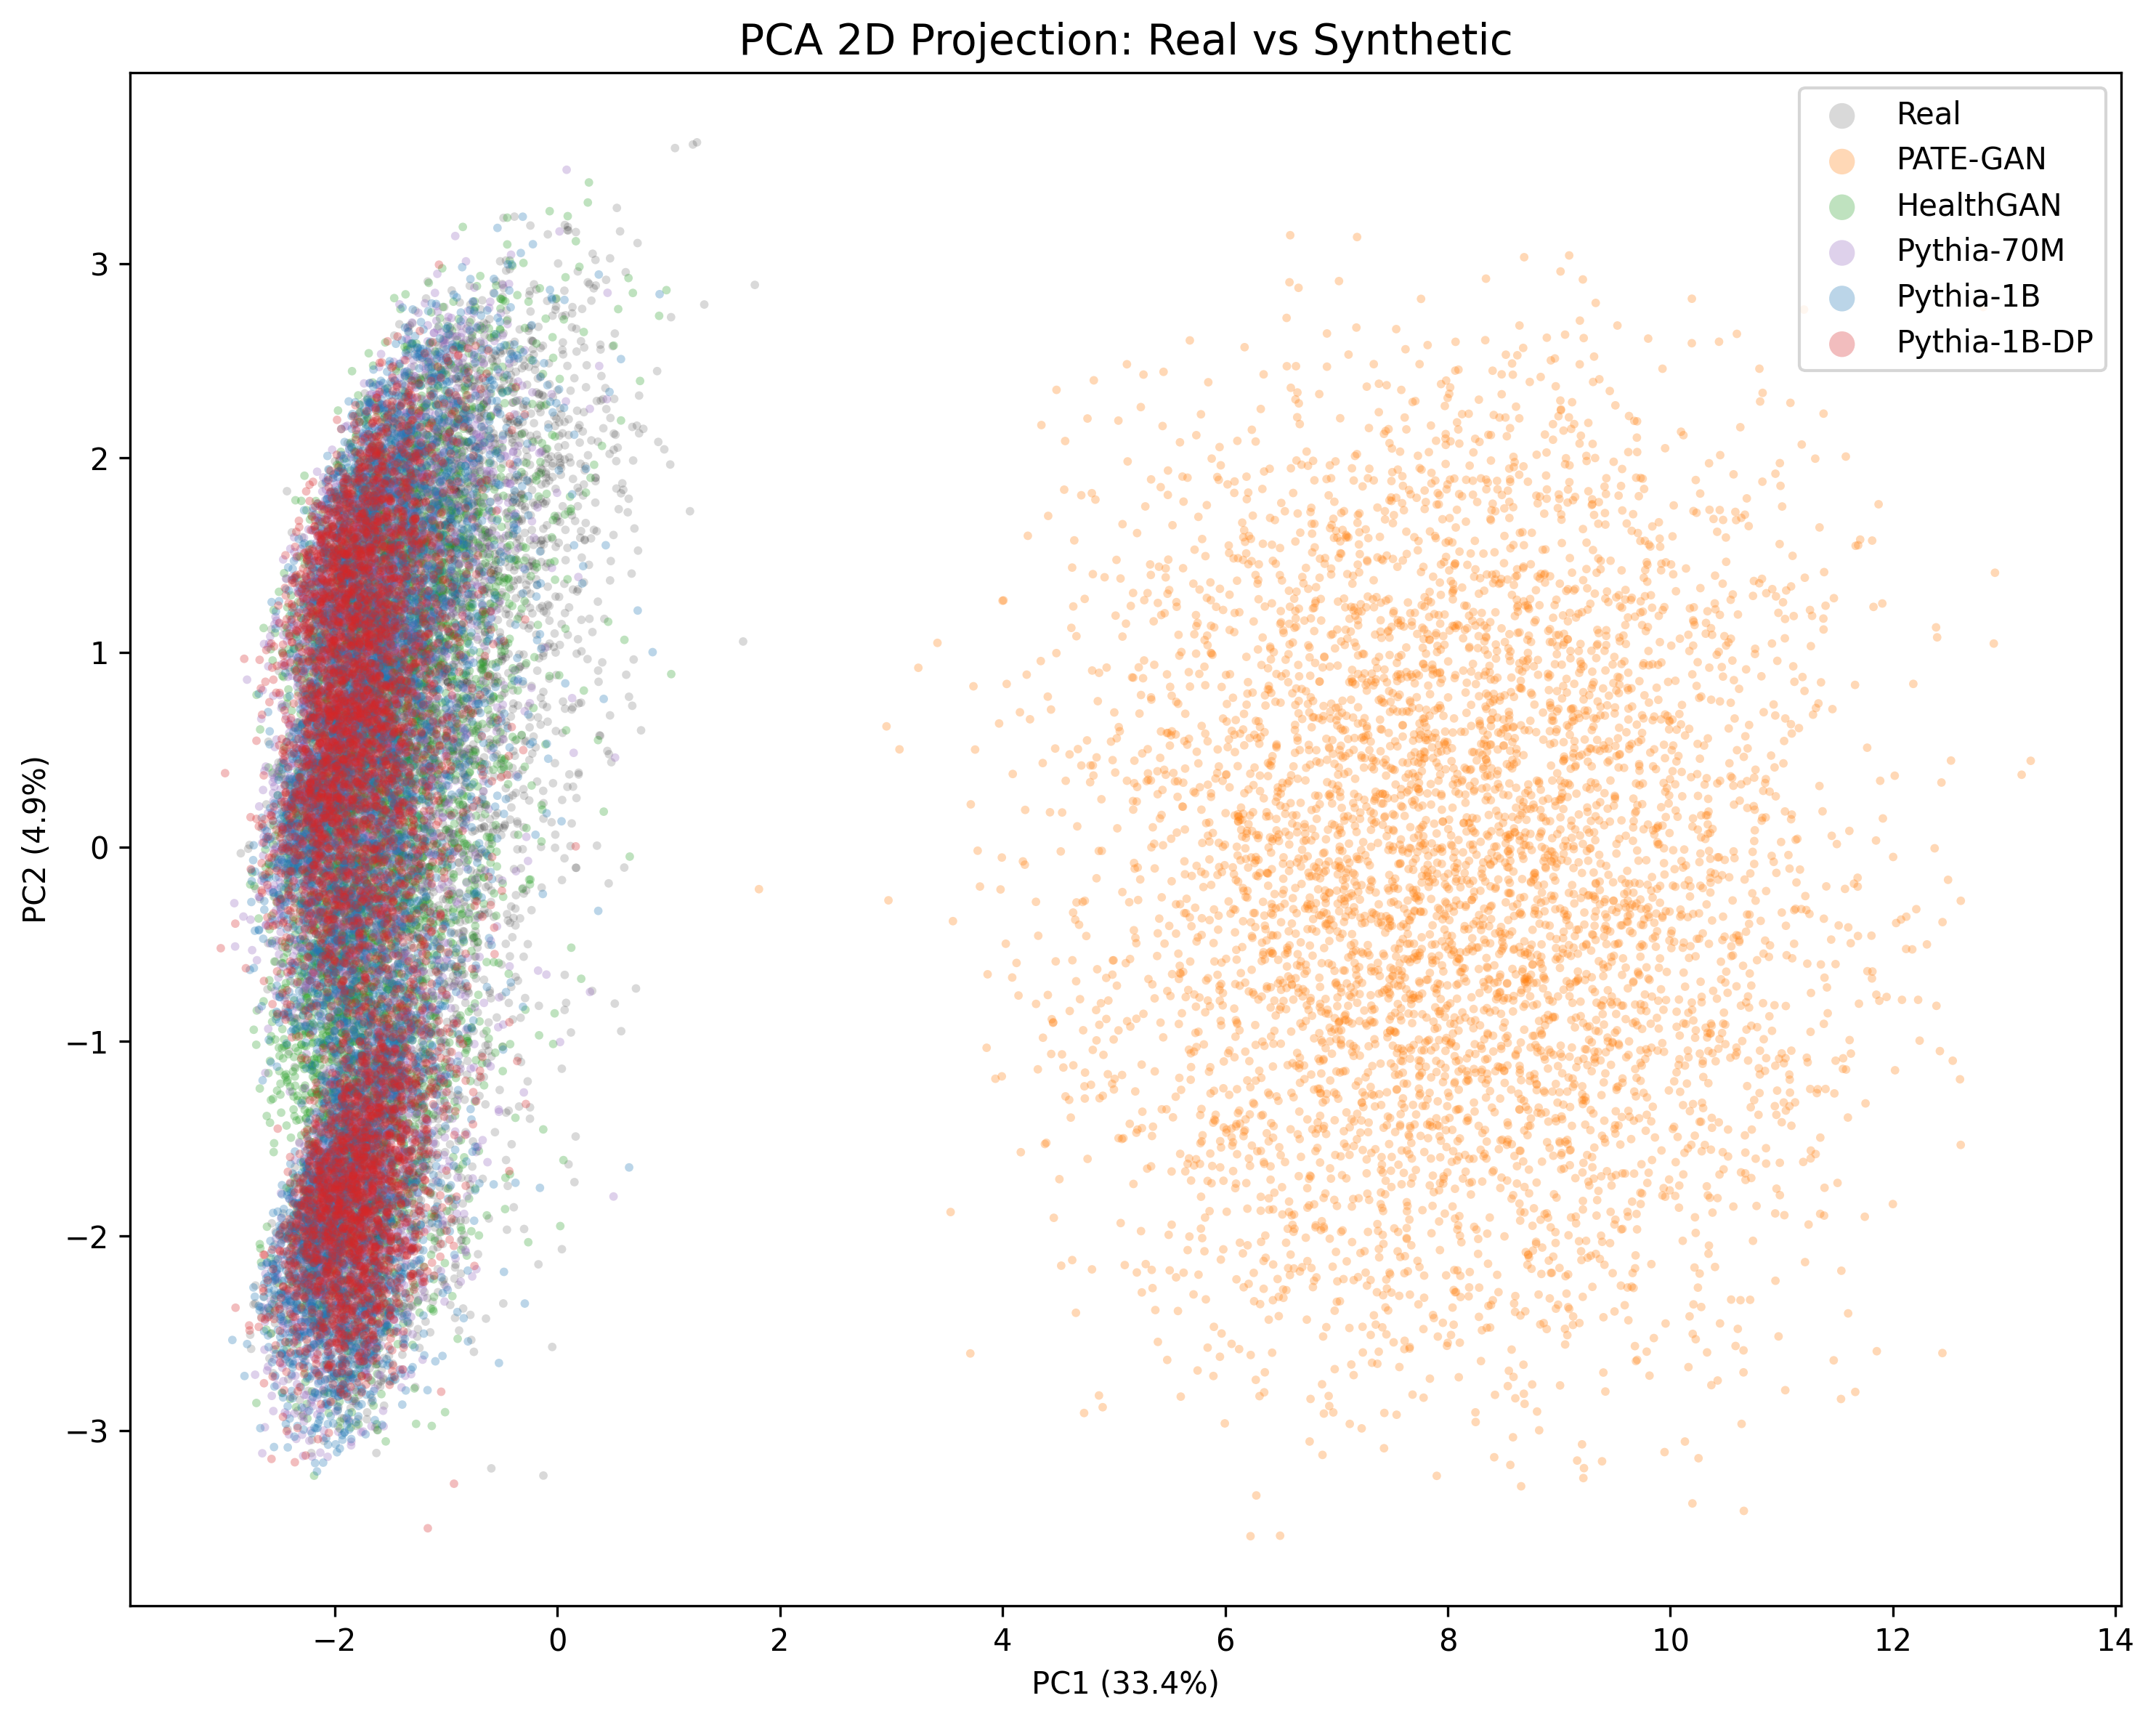
\includegraphics[width=0.85\textwidth]{images/results/1e-pca_projection}
\caption{Two-dimensional PCA projection onto principal components estimated
from the combined real-plus-synthetic table. Four generators overlap the
real cloud; PATE-GAN is displaced into a disjoint region along the first
principal component.}
\label{fig:rq2:pca}
\end{figure}

\subsubsection{Predictive Performance}
\label{sec:results:rq2:utility:predictive}

Predictive utility is measured under the Train-on-Synthetic,
Test-on-Real (TSTR) protocol defined in
Section~\ref{sec:eval:utility:predictive:tstr}. A classifier is trained
on each synthetic table and evaluated on the held-out real test split
($n = 14{,}304$) with \emph{readmitted} as the binary target. The
Train-on-Real, Test-on-Real (TRTR) model provides the upper-bound
reference. Three downstream classifiers are reported
(Section~\ref{sec:eval:utility:predictive:classifiers}). Gradient
Boosting is taken as the headline model, with Logistic Regression and
Random Forest included.

\paragraph{Class-Balance Diagnostic:}
Before interpreting the threshold-dependent classifier metrics, the
positive-class prevalence of the binary readmission target was checked
across real and synthetic train/test splits. The real train and test splits
both have a readmission rate of approximately $0.340$. PATE-GAN
substantially over-produces the positive class in both synthetic splits
($0.498$ train, $0.507$ test), whereas HealthGAN remains close to the real
prevalence and the Pythia variants match the real split proportions by
construction through class-conditioned generation. This diagnostic is not a
predictive-utility metric, but it helps interpret F1, precision, and recall,
because target-prevalence shifts can change classifier operating behaviour
independently of feature quality. The full class-balance table and
TRTR/TSTR/TRTS/TSTS AUC-ROC matrix are reported in
Appendix~\ref{app:class-balance}.

\paragraph{TSTR Classifier Performance:}
Table~\ref{tab:rq2:tstr} presents the TSTR results for every combination
of training source and classifier. Models trained on real data are
included as a reference. Based on Gradient-Boosting AUC-ROC, Pythia-1B
achieves the best synthetic-data result $(0.6818)$, followed by
Pythia-70M, HealthGAN, Pythia-1B-DP,
and PATE-GAN. The real-trained model achieves $0.7008$.
Pythia-1B therefore retains approximately $97\%$ of the real-data
AUC-ROC, while PATE-GAN performs only slightly above the chance level
of $0.5$. This means that Pythia-1B preserves most of the predictive
information available in the real data, whereas PATE-GAN preserves
little useful discriminatory information.

\begin{table}[H]
\centering
\small
\caption{Train-on-Synthetic, Test-on-Real (TSTR) utility for all five
generators and the Train-on-Real (TRTR) reference, evaluated on the real
held-out split ($n = 14{,}304$) with \emph{readmitted} as the target.
The highest synthetic Gradient-Boosting AUC-ROC is shown in bold.}
\label{tab:rq2:tstr}
% Auto-generated by data_analysis.ipynb (2a). Do not edit by hand.
% Requires booktabs.
\begin{tabular}{llccccc}
\toprule
Train Source & Classifier & AUC-ROC & F1 & Accuracy & Precision & Recall \\
\midrule
Real (TRTR) & Logistic Regression & 0.6670 & 0.2837 & 0.6804 & 0.5974 & 0.1860 \\
Real (TRTR) & Random Forest & 0.6790 & 0.3648 & 0.6895 & 0.6000 & 0.2620 \\
Real (TRTR) & Gradient Boosting & 0.7008 & 0.3668 & 0.6962 & 0.6301 & 0.2587 \\
\midrule
PATE-GAN & Logistic Regression & 0.5079 & 0.0417 & 0.6528 & 0.3407 & 0.0222 \\
PATE-GAN & Random Forest & 0.5018 & 0.0246 & 0.6567 & 0.3669 & 0.0127 \\
PATE-GAN & Gradient Boosting & 0.5108 & 0.0093 & 0.6583 & 0.3433 & 0.0047 \\
\midrule
HealthGAN & Logistic Regression & 0.6130 & 0.3889 & 0.6651 & 0.5128 & 0.3132 \\
HealthGAN & Random Forest & 0.6153 & 0.3826 & 0.6655 & 0.5142 & 0.3046 \\
HealthGAN & Gradient Boosting & 0.6312 & 0.3824 & 0.6720 & 0.5321 & 0.2984 \\
\midrule
Pythia-70M & Logistic Regression & 0.6573 & 0.5035 & 0.6337 & 0.4671 & 0.5460 \\
Pythia-70M & Random Forest & 0.6588 & 0.4966 & 0.6442 & 0.4787 & 0.5158 \\
Pythia-70M & Gradient Boosting & 0.6634 & 0.5005 & 0.6408 & 0.4749 & 0.5290 \\
\midrule
Pythia-1B & Logistic Regression & 0.6613 & 0.4984 & 0.6393 & 0.4730 & 0.5267 \\
Pythia-1B & Random Forest & 0.6682 & 0.5048 & 0.6523 & 0.4896 & 0.5210 \\
Pythia-1B & Gradient Boosting & \textbf{0.6818} & 0.5036 & 0.6569 & 0.4959 & 0.5115 \\
\midrule
Pythia-1B-DP & Logistic Regression & 0.5868 & 0.2509 & 0.6477 & 0.4535 & 0.1734 \\
Pythia-1B-DP & Random Forest & 0.5823 & 0.2369 & 0.6456 & 0.4426 & 0.1617 \\
Pythia-1B-DP & Gradient Boosting & 0.5827 & 0.2714 & 0.6389 & 0.4327 & 0.1977 \\
\bottomrule
\end{tabular}

\end{table}

The F1 scores show a different pattern. HealthGAN and the two
non-private Pythia models exceed the real-trained F1 score of $0.3668$,
with both Pythia models achieving approximately $0.50$. For the
non-private Pythia models, recall increases from approximately $0.26$
to between $0.51$ and $0.53$, while precision decreases from $0.63$
to between $0.47$ and $0.50$. This means that their higher F1 scores
result from identifying more readmitted patients, but at the cost of
producing more false-positive predictions. Their lower AUC-ROC values
show that this does not represent better overall discrimination than
the real-trained model.

Pythia-1B-DP achieves a lower F1 score of $0.2714$. PATE-GAN performs
poorly on both measures. Its Gradient-Boosting F1 score of $0.0093$ and
recall of $0.0047$ show that the classifier rarely predicts the positive
class. This means that differential privacy reduces the predictive
utility of Pythia-1B in this evaluation, while PATE-GAN produces
synthetic data with very limited usefulness for the readmission task.
Overall, AUC-ROC and F1 describe different aspects of predictive
utility, consistent with Table~\ref{tab:rq1-coverage}.


\paragraph{ROC Curves:}
Figure~\ref{fig:rq2:roc} overlays the Gradient-Boosting ROC curves of all
five generators against the real reference. The curves recover the AUC
ordering of Table~\ref{tab:rq2:tstr} visually. The real curve (AUC
$0.701$) has the highest AUC. Pythia-1B ($0.682$) and Pythia-70M
($0.663$) lie just beneath it. HealthGAN ($0.631$) is lower and then Pythia-1B-DP
($0.583$). PATE-GAN ($0.511$) tracks the chance diagonal
across almost the entire false-positive range.

\begin{figure}[H]
\centering
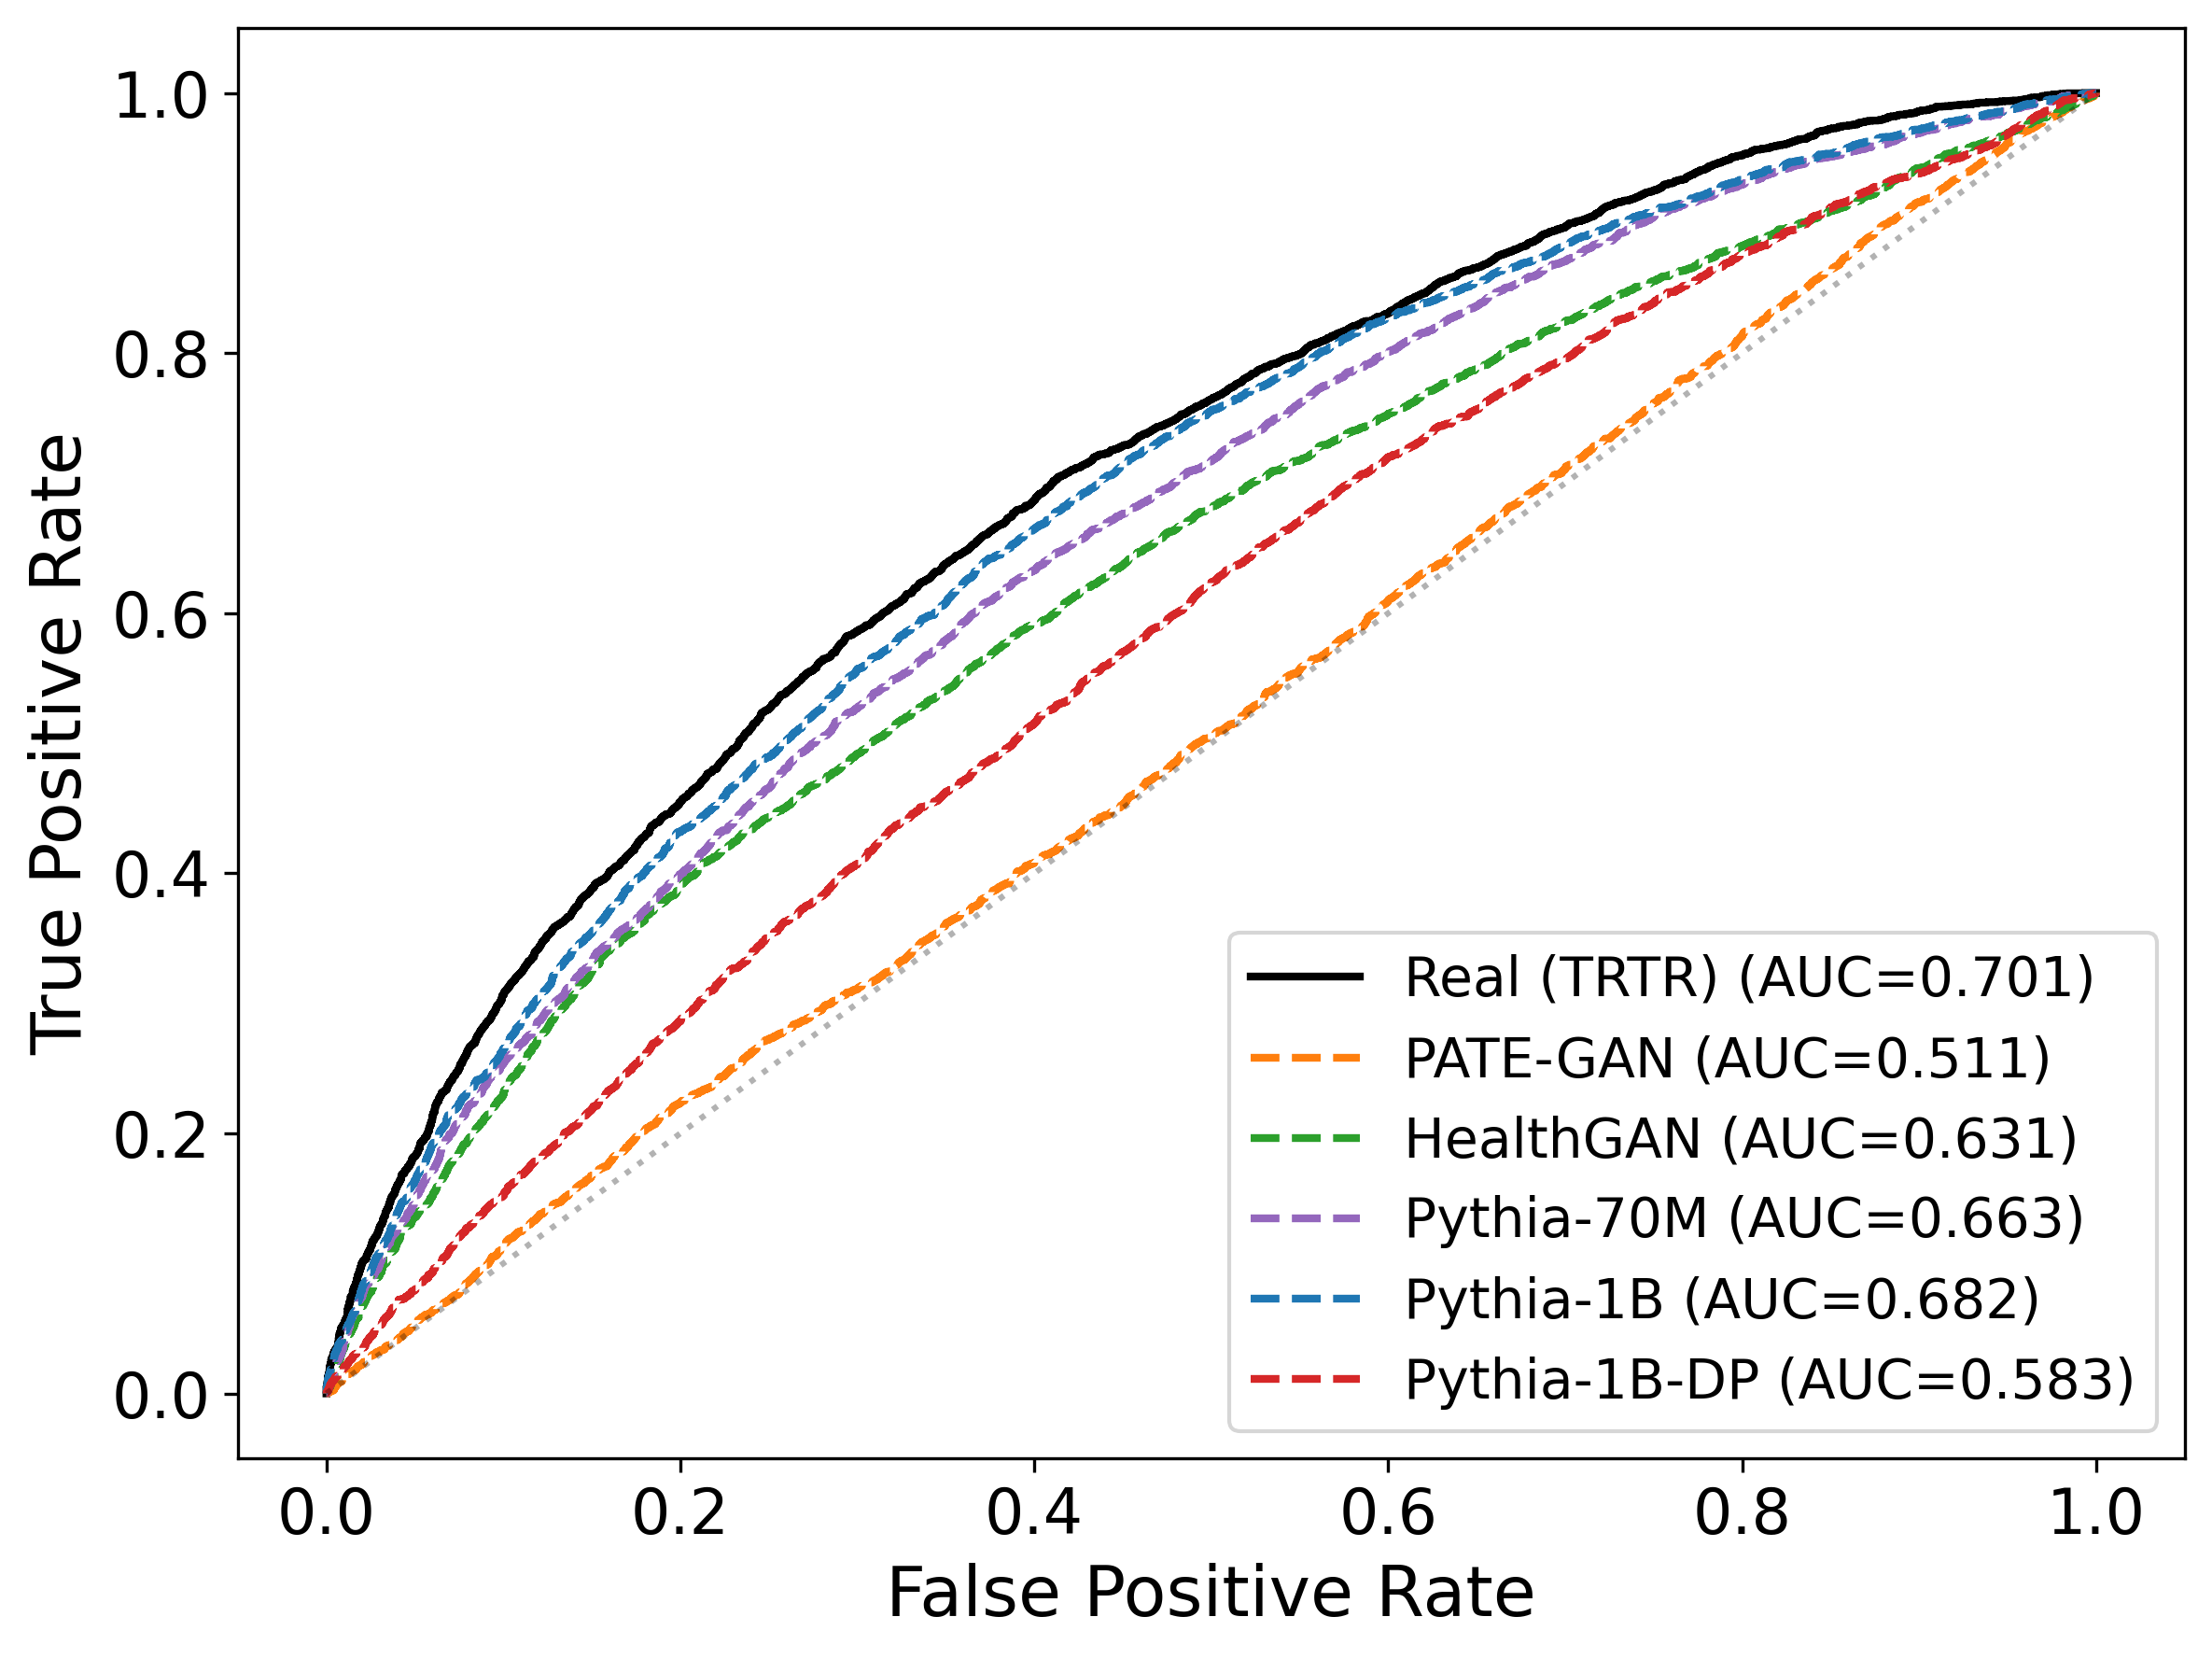
\includegraphics[width=0.75\textwidth]{images/results/2b-roc_curves}
\caption{Gradient-Boosting ROC curves under TSTR for all five generators
and the real (TRTR) reference. Legend values are the corresponding
AUC-ROC scores.}
\label{fig:rq2:roc}
\end{figure}

\paragraph{Feature-Importance Stability:}
Figure~\ref{fig:rq2:featimp} reports the feature-importance agreement
score defined in Section~\ref{sec:eval:utility:predictive:fi}. The score
compares the normalised random-forest importance vector obtained from each
synthetic-trained model with the real-trained reference. Here, 
higher values indicate a more similar distribution of importance
across the engineered features. HealthGAN ($0.914$), Pythia-1B ($0.911$), Pythia-70M ($0.889$),
and Pythia-1B-DP ($0.856$) remain close to the real reference, whereas
PATE-GAN is lower ($0.675$). This suggests that the four non-PATE
generators retain a broadly similar model-based importance profile, while
PATE-GAN departs more strongly. This diagnostic assesses model-specific 
predictive patterns, not as evidence that the
identified predictors are causal or clinically validated. The corresponding
top-ranked features and the PATE-GAN-specific divergence pattern are shown
in Appendix~\ref{app:feature-importance}.

\begin{figure}[!htbp]
\centering
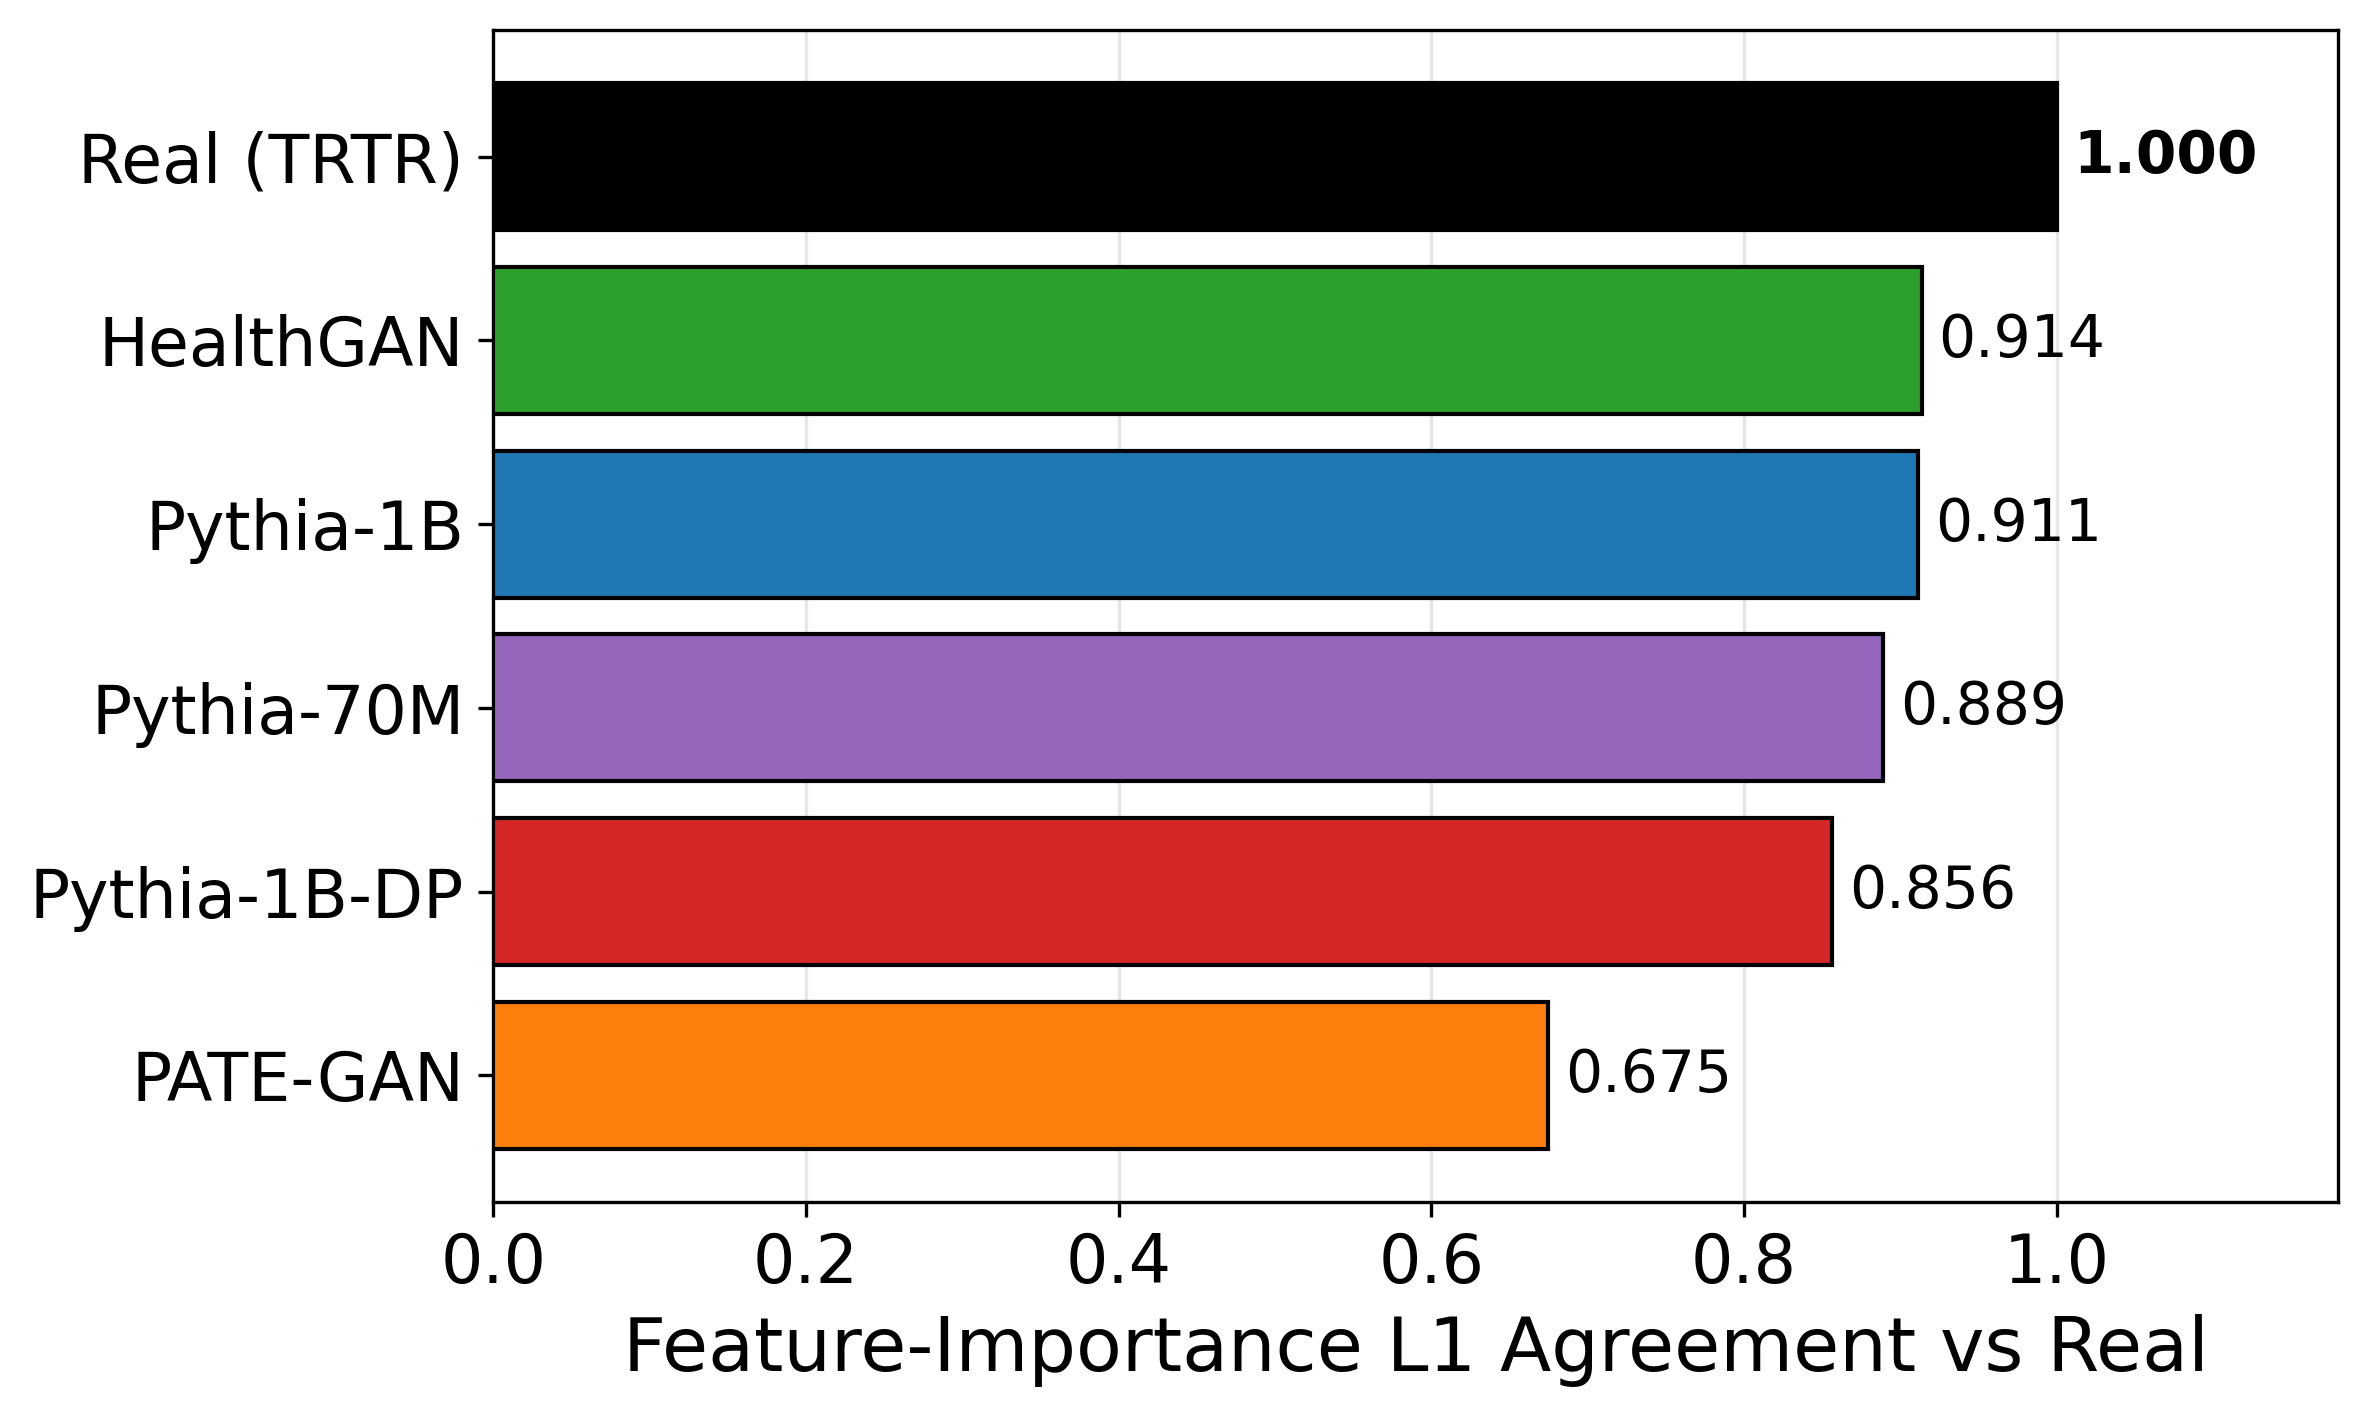
\includegraphics[width=0.76\textwidth]{images/results/2c_ii-feature_importance_l1}
\caption{Feature-importance agreement with the real-trained random-forest
reference. Scores are based on the $L_1$ distance between normalised
importance vectors; higher values indicate closer agreement.}
\label{fig:rq2:featimp}
\end{figure}

\paragraph{Cox Proportional-Hazards Agreement:}
Agreement on a Cox proportional-hazards model
(Section~\ref{sec:eval:utility:predictive:cox}) tests whether the
synthetic data preserve survival-style association patterns. A Cox model is
fitted on each data source. Agreement is
measured by counting the covariates whose synthetic $95\%$ hazard-ratio
confidence intervals overlap the corresponding real-data intervals.
(Section~\ref{sec:eval:utility:predictive:cox-overlap}). The overlap
summary in Table~\ref{tab:rq2:cox} is used as the main result because it is
the scalar Cox metric defined in the methodology. The full per-covariate
hazard-ratio plots are provided in Appendix~\ref{app:cox}.

HealthGAN and the two 1B-parameter Pythia variants show the strongest
agreement on this metric, with seven overlapping covariates each
(HealthGAN: $7/12$; Pythia-1B and Pythia-1B-DP: $7/13$). 
HealthGAN is evaluated on twelve covariates because
\emph{number\_emergency} has zero variance in its synthetic data and was
therefore excluded from the Cox model. Pythia-70M
overlaps on four of thirteen covariates, while PATE-GAN overlaps on none.
The identical overlap counts for Pythia-1B and Pythia-1B-DP indicate that
the utility loss observed under TSTR AUC-ROC is not mirrored by this
coarser Cox-overlap diagnostic. PATE-GAN's result also aligns with our finding 
of distorted dataset generation in this evaluation as well.
This should be read as agreement in fitted
Cox effect-size intervals, not as evidence that the synthetic data validate
clinical causal relationships.

\begin{table}[H]
\centering
\small
\caption{Cox proportional-hazards confidence-interval overlap per
generator: the number of covariates whose synthetic $95\%$ hazard-ratio
interval overlaps the real interval, out of those fitted (higher is
better). HealthGAN is fitted on twelve covariates because one
zero-variance column was dropped.}
\label{tab:rq2:cox}
% Auto-generated by data_analysis.ipynb (2e). Do not edit by hand.
% Requires booktabs.
\begin{tabular}{lcc}
\toprule
Generator & CIs overlapping & Fraction $\uparrow$ \\
\midrule
PATE-GAN & 0 / 13 & 0.000 \\
HealthGAN & 7 / 12 & 0.583 \\
Pythia-70M & 4 / 13 & 0.308 \\
Pythia-1B & 7 / 13 & 0.538 \\
Pythia-1B-DP & 7 / 13 & 0.538 \\
\bottomrule
\end{tabular}

\end{table}

\subsubsection{Ablation: Age Binning Granularity}
\label{sec:results:rq2:utility:age-binning}

The preprocessing pipeline (Section~\ref{sec:data:fe:age}) retains the
dataset's original ten age categories. An earlier approach that grouped
age into three broader categories (young, middle-aged, and elderly) was
not used. Table~\ref{tab:age-binning-tstr} quantifies the impact on
Train-on-Synthetic, Test-on-Real (TSTR) utility for the three generators
with matched runs under both age encodings: PATE-GAN, HealthGAN, and
Pythia-70M. The ablation is therefore a preprocessing-sensitivity check,
not a full five-generator comparison. Pythia-1B and Pythia-1B-DP are not
included because they were introduced after the preprocessing pipeline had
already been revised to the retained ten-bin age encoding. No matched
three-bin runs are available for those models. All evaluations use the
real held-out test split ($n = 14{,}304$) with \emph{readmitted} as the
binary target. Gradient Boosting is used as the primary downstream classifier.
Logistic Regression and Random Forest show similar overall patterns.
\vspace{0.5em}

\begin{table}[H]
\centering
\small
\caption{TSTR utility under the discarded three-bin age encoding versus
the retained ten-bin encoding. Test set: real held-out split
($n = 14{,}304$); target: \emph{readmitted}; classifier: Gradient
Boosting. $\Delta$ is computed as the difference from 10-bin value to the 3-bin
value.}
\label{tab:age-binning-tstr}
\begin{tabular}{llccc}
\toprule
Train Source & Metric & 3-bin & 10-bin & $\Delta$ \\
\midrule
Real (TRTR) & AUC-ROC & 0.7014 & 0.7008 & $-0.0006$ \\
Real (TRTR) & F1      & 0.3644 & 0.3668 & $+0.0024$ \\
\midrule
PATE-GAN    & AUC-ROC & 0.4823 & 0.5108 & $+0.0285$ \\
PATE-GAN    & F1      & 0.0437 & 0.0093 & $-0.0344$ \\
HealthGAN   & AUC-ROC & 0.6605 & 0.6312 & $-0.0293$ \\
HealthGAN   & F1      & 0.2647 & 0.3824 & $+0.1177$ \\
Pythia-70M  & AUC-ROC & 0.5981 & \textbf{0.6634} & $\mathbf{+0.0653}$ \\
Pythia-70M  & F1      & 0.3944 & \textbf{0.5005} & $\mathbf{+0.1061}$ \\
\bottomrule
\end{tabular}
\end{table}

The Train-on-Real Test-on-Real is essentially unchanged between the two
encodings, indicating that the ablation does not alter the real-data
prediction task in a meaningful way. Within the matched generators,
however, the effect is model-dependent. Pythia-70M improves most under
the retained ten-bin encoding (AUC-ROC $+0.0653$; F1 $+0.1061$),
suggesting that the token-based generator benefited from the more detailed
age representation. HealthGAN shows a mixed response: AUC-ROC is higher
under the discarded three-bin encoding, whereas F1 is higher under the
retained ten-bin encoding. PATE-GAN remains weak under both settings, so
age granularity is unlikely to be its primary utility bottleneck in this
experiment. Overall, the ablation supports the ten-bin preprocessing
choice while showing that age encoding can affect generators differently.

% ROC, feature-importance, and Cox predictive results are reported above
% within Predictive Performance (§\ref{sec:results:rq2:utility:predictive});
% the age-binning ablation is a preprocessing-sensitivity finding kept as
% the final subsubsection of the utility results.

\subsection{Privacy Results}
\label{sec:results:rq2:privacy}

Privacy is assessed using the empirical metrics defined in
Section~\ref{sec:eval:privacy}. These include distance-based proximity
measures, outlier-linkability analysis, and inference-attack
simulations. Each metric examines a specific disclosure risk and does
not independently provide a formal privacy guarantee. The privacy
results are therefore interpreted together and alongside the utility
results, since synthetic data that depart substantially from the real
distribution may appear private under distance-based measures. Selected
privacy diagnostics are summarised in Figure~\ref{fig:rq2:privacy}.

\paragraph{Nearest-Neighbour Distance and Distance Ratio:}
Table~\ref{tab:rq2:nn} presents the median and fifth-percentile
nearest-neighbour distances in both directions for each generator. It
also reports the NNDR defined in
Section~\ref{sec:eval:privacy:nn}. The median represents typical record
proximity. In the synthetic-to-real direction, the fifth percentile
focuses on the lower tail of records closest to the real data and is
therefore more relevant to disclosure risk. An NNDR close to one
indicates that synthetic-to-real proximity is similar to the spacing
between real records. It is important to note that, NNDR is a proximity diagnostic and does
not independently demonstrate privacy.

\begin{table}[H]
\centering
\small
\caption{Median and fifth-percentile nearest-neighbour distances and
median NNDR for each generator. The fifth-percentile synthetic-to-real
distance describes the lower proximity tail. The median real-to-real
nearest-neighbour distance is $2.019$ and is included as a descriptive
reference. Larger synthetic-to-real distances and
$\text{NNDR} \geq 1$ suggest lower proximity risk only when the
synthetic data also preserve the real-data distribution.}
\label{tab:rq2:nn}
% Auto-generated by data_analysis.ipynb (3a). Do not edit by hand.
% Requires booktabs.
\begin{tabular}{lccccc}
\toprule
 & R$\rightarrow$S median & R$\rightarrow$S 5th pct & S$\rightarrow$R median & S$\rightarrow$R 5th pct & NNDR median \\
\midrule
PATE-GAN & 41.268 & 39.706 & 219.879 & 79.995 & 104.601 \\
HealthGAN & 2.924 & 1.439 & 2.233 & 1.136 & 1.063 \\
Pythia-70M & 2.684 & 1.140 & 1.440 & 0.771 & 0.721 \\
Pythia-1B & 2.581 & 1.060 & 1.406 & 0.727 & 0.698 \\
Pythia-1B-DP & 2.811 & 1.217 & 1.533 & 0.833 & 0.763 \\
\bottomrule
\end{tabular}

\end{table}

The four non-PATE generators produce synthetic records at distances
comparable to the typical spacing between real records. HealthGAN has
a median synthetic-to-real distance of $2.233$ and an NNDR of $1.063$,
both close to the real-to-real reference. The three Pythia variants
have lower median distances of $1.406$-$1.533$ and NNDR values of
$0.698$-$0.763$. This indicates that their synthetic records are
typically closer to the real data than real records are to one another.
However, this proximity alone does not justify that records were
copied.

PATE-GAN produces a much larger median synthetic-to-real distance of
$219.879$ and an NNDR of $104.601$. Given its poor similarity results
in Section~\ref{sec:results:rq2:utility:similarity}, these values indicate
that its records have moved away from the real-data distribution. They
should therefore be interpreted as poor fidelity rather than strong
privacy protection. This result demonstrates why distance-based privacy
metrics must be considered together with utility and fidelity measures.

For the four non-PATE generators, the fifth-percentile
synthetic-to-real distances range from $0.727$ to $1.136$. These
positive values indicate that the lower proximity tail generally
remains separated from the real data. However, a positive fifth
percentile cannot exclude rarer exact or near-exact matches below that
percentile. Together with the NNAA and membership-inference results in
Sections~\ref{sec:results:rq2:privacy:nnaa}
and~\ref{sec:results:rq2:privacy:mia}, the findings provide no evidence
of widespread training-record memorisation. PATE-GAN's
fifth-percentile distance of $79.995$ reflects the same distributional
drift as its median and should not be interpreted as evidence of
effective privacy protection.

\paragraph{Nearest-Neighbour Adversarial Accuracy:}
\label{sec:results:rq2:privacy:nnaa}

Nearest-neighbour adversarial accuracy (NNAA) in
Section~\ref{sec:eval:privacy:nnaa} is calculated separately for the
training and test sets. The ideal value for both TrainAA and TestAA is
$0.5$, indicating that the adversary performs no better than random
guessing when distinguishing synthetic from real records. Privacy loss is
calculated as the difference between TestAA and TrainAA, with a value near
zero indicating little evidence of training-set memorisation.
Table~\ref{tab:rq2:nnaa} reports these three values.

\begin{table}[H]
\centering
\small
\caption{Nearest-neighbour adversarial accuracy per generator. Train and
test adversarial accuracy near $0.5$ indicates good resemblance. Privacy
loss (test $-$ train) near $0.0$ indicates no memorisation.}
\label{tab:rq2:nnaa}
% Auto-generated by data_analysis.ipynb (3a_ii). Do not edit by hand.
% Requires booktabs.
\begin{tabular}{lccc}
\toprule
Generator & Train AA & Test AA & Privacy loss \\
\midrule
PATE-GAN & 1.0000 & 0.9999 & $-0.0001$ \\
HealthGAN & 0.7182 & 0.7199 & $+0.0017$ \\
Pythia-70M & 0.6469 & 0.6499 & $+0.0030$ \\
Pythia-1B & 0.6207 & 0.6204 & $-0.0003$ \\
Pythia-1B-DP & 0.7063 & 0.7139 & $+0.0076$ \\
\bottomrule
\end{tabular}

\end{table}

Privacy loss is close to zero for all generators, ranging from $-0.0001$
to $+0.0076$. This provides no meaningful evidence that the generators
reproduce training records more closely than held-out records. PATE-GAN's
NNAA of approximately $1.0$ shows that its synthetic data are easily
distinguishable from the real data, whereas the other generators achieve
values between $0.62$ and $0.72$. Pythia-1B is closest to the ideal value
of $0.5$ ($0.621$), although all generators remain distinguishable from
the real data. Overall, the near-zero privacy loss suggests that this
distinguishability is not caused by training-set memorisation.

\paragraph{Membership Inference:}
\label{sec:results:rq2:privacy:mia}

A distance-based membership-inference adversary
(Section~\ref{sec:eval:privacy:mia}) attempts to decide whether a given
real record was part of the generator's training set.
Table~\ref{tab:rq2:mia} reports the AUC-ROC achieved by the membership-inference attack.

\begin{table}[H]
\centering
\small
\caption{Membership-inference attack results per generator. AUC near
$0.5$ and advantage near $0.0$ indicate that the adversary cannot
distinguish training members from non-members.}
\label{tab:rq2:mia}
% Auto-generated by data_analysis.ipynb (3b). Do not edit by hand.
% Requires booktabs.
\begin{tabular}{lcc}
\toprule
Generator & MIA AUC & MIA advantage \\
\midrule
PATE-GAN & 0.4984 & $-0.0016$ \\
HealthGAN & 0.5005 & $+0.0005$ \\
Pythia-70M & 0.5119 & $+0.0119$ \\
Pythia-1B & 0.4926 & $-0.0074$ \\
Pythia-1B-DP & 0.4931 & $-0.0069$ \\
\bottomrule
\end{tabular}

\end{table}

Membership-inference performance remains close to random guessing across
all generators. Every attack AUC lies within $[0.493, 0.512]$ of the
random-guess baseline, and every advantage is within $\pm 0.012$ of zero.
The largest signal, Pythia-70M's AUC of
$0.512$, remains negligible. No generator, private or otherwise, shows
evidence of exploitable membership leakage under this distance-based
adversary. This is consistent with the absence of memorisation indicated
by the privacy-loss measure above.

\paragraph{Attribute Inference:}
\label{sec:results:rq2:privacy:aia}

The attribute-inference attack
(Section~\ref{sec:eval:privacy:aia}) evaluates whether a predictor trained
on synthetic data can recover sensitive attributes from real records more
accurately than a marginal baseline. Table~\ref{tab:rq2:aia} reports 
the per-attribute advantage for
the four attributes considered. The final column reports the 
maximum advantage for each generator and is
used in the comprehensive summary.

\begin{table}[H]
\centering
\small
\caption{Attribute-inference advantage per generator and attribute
(positive values indicate leakage above the marginal baseline). The
final column is the per-generator maximum advantage.}
\label{tab:rq2:aia}
% Auto-generated by data_analysis.ipynb (3c). Do not edit by hand.
% Requires booktabs.
\begin{tabular}{lccccc}
\toprule
Generator & \texttt{readmitted} & \texttt{gender} & \texttt{age} & \texttt{diag\_1} & Max \\
\midrule
PATE-GAN & $-0.3334$ & $-0.0560$ & $-0.0266$ & $-0.2330$ & $-0.0266$ \\
HealthGAN & $-0.0046$ & $-0.0040$ & $-0.0338$ & $-0.0218$ & $-0.0040$ \\
Pythia-70M & $-0.0236$ & $-0.0052$ & $-0.0332$ & $+0.0064$ & $+0.0064$ \\
Pythia-1B & $-0.0168$ & $+0.0104$ & $+0.0024$ & $+0.0410$ & $+0.0410$ \\
Pythia-1B-DP & $-0.0296$ & $-0.0056$ & $-0.0322$ & $-0.0166$ & $-0.0056$ \\
\bottomrule
\end{tabular}

\end{table}

Most advantage values are zero or negative, indicating that the attack
does not outperform the marginal baseline. Pythia-1B is the main
exception, showing a small positive advantage for the primary diagnosis
(\emph{diag\_1}, $+0.0410$) and smaller advantages for \emph{gender} and
\emph{age}. This signal is absent in Pythia-1B-DP, whose \emph{diag\_1}
advantage is $-0.0166$ and maximum advantage is $-0.0056$. This represents
the main privacy improvement of differential privacy within the LLM
family and is examined further in
Section~\ref{sec:results:rq3:llm-toggle}. PATE-GAN's strongly negative
values for \emph{readmitted} ($-0.3334$) and \emph{diag\_1} ($-0.2330$)
reflect its limited data quality rather than stronger privacy protection.

\paragraph{Outlier Linkability:}
\label{sec:results:rq2:privacy:linkability}

The clustering-proximity test
(Section~\ref{sec:eval:privacy:linkability}) evaluates disclosure risk
for unusual real records. It compares the percentage of outliers and
non-outliers that have a nearby synthetic record within a radius of
$2.636$, corresponding to the $75^{\text{th}}$ percentile of real-to-real
nearest-neighbour distances. The $5\%$ of real records farthest from the
data centroid ($2{,}861$ records) are defined as outliers.
Table~\ref{tab:rq2:linkability} reports both percentages and their
difference.

\begin{table}[H]
\centering
\small
\caption{Outlier versus non-outlier linkability per generator (percentage
of real records with a synthetic neighbour within radius $2.636$). Low
outlier linkability indicates that the generator does not concentrate mass
around vulnerable records; a positive gap indicates coverage of common
rather than extreme patterns. The gap is reported in percentage points.}
\label{tab:rq2:linkability}
% Auto-generated by data_analysis.ipynb (3d). Do not edit by hand.
% Requires booktabs.
\begin{tabular}{lccc}
\toprule
Generator & Outlier \% & Non-outlier \% & Gap (pp) \\
\midrule
PATE-GAN & 0.0 & 0.0 & $+0.0$ \\
HealthGAN & 0.0 & 42.0 & $+42.0$ \\
Pythia-70M & 0.1 & 50.6 & $+50.6$ \\
Pythia-1B & 0.6 & 53.3 & $+52.6$ \\
Pythia-1B-DP & 0.0 & 46.8 & $+46.8$ \\
\bottomrule
\end{tabular}

\end{table}

Outlier linkability is near zero for every generator (at most $0.6\%$, for
Pythia-1B), indicating that very few vulnerable tail records have a nearby
synthetic neighbour. The non-collapsed generators link a substantial
fraction of non-outliers ($42$-$53\%$). The resulting large positive
gap is consistent with the intended pattern. Common clinical regions are
covered while rare, identifiable records remain largely uncovered.
PATE-GAN links neither outliers nor non-outliers
($0\%$ on both), consistent with output that lies away from the real
manifold altogether.

\begin{figure}[H]
\centering
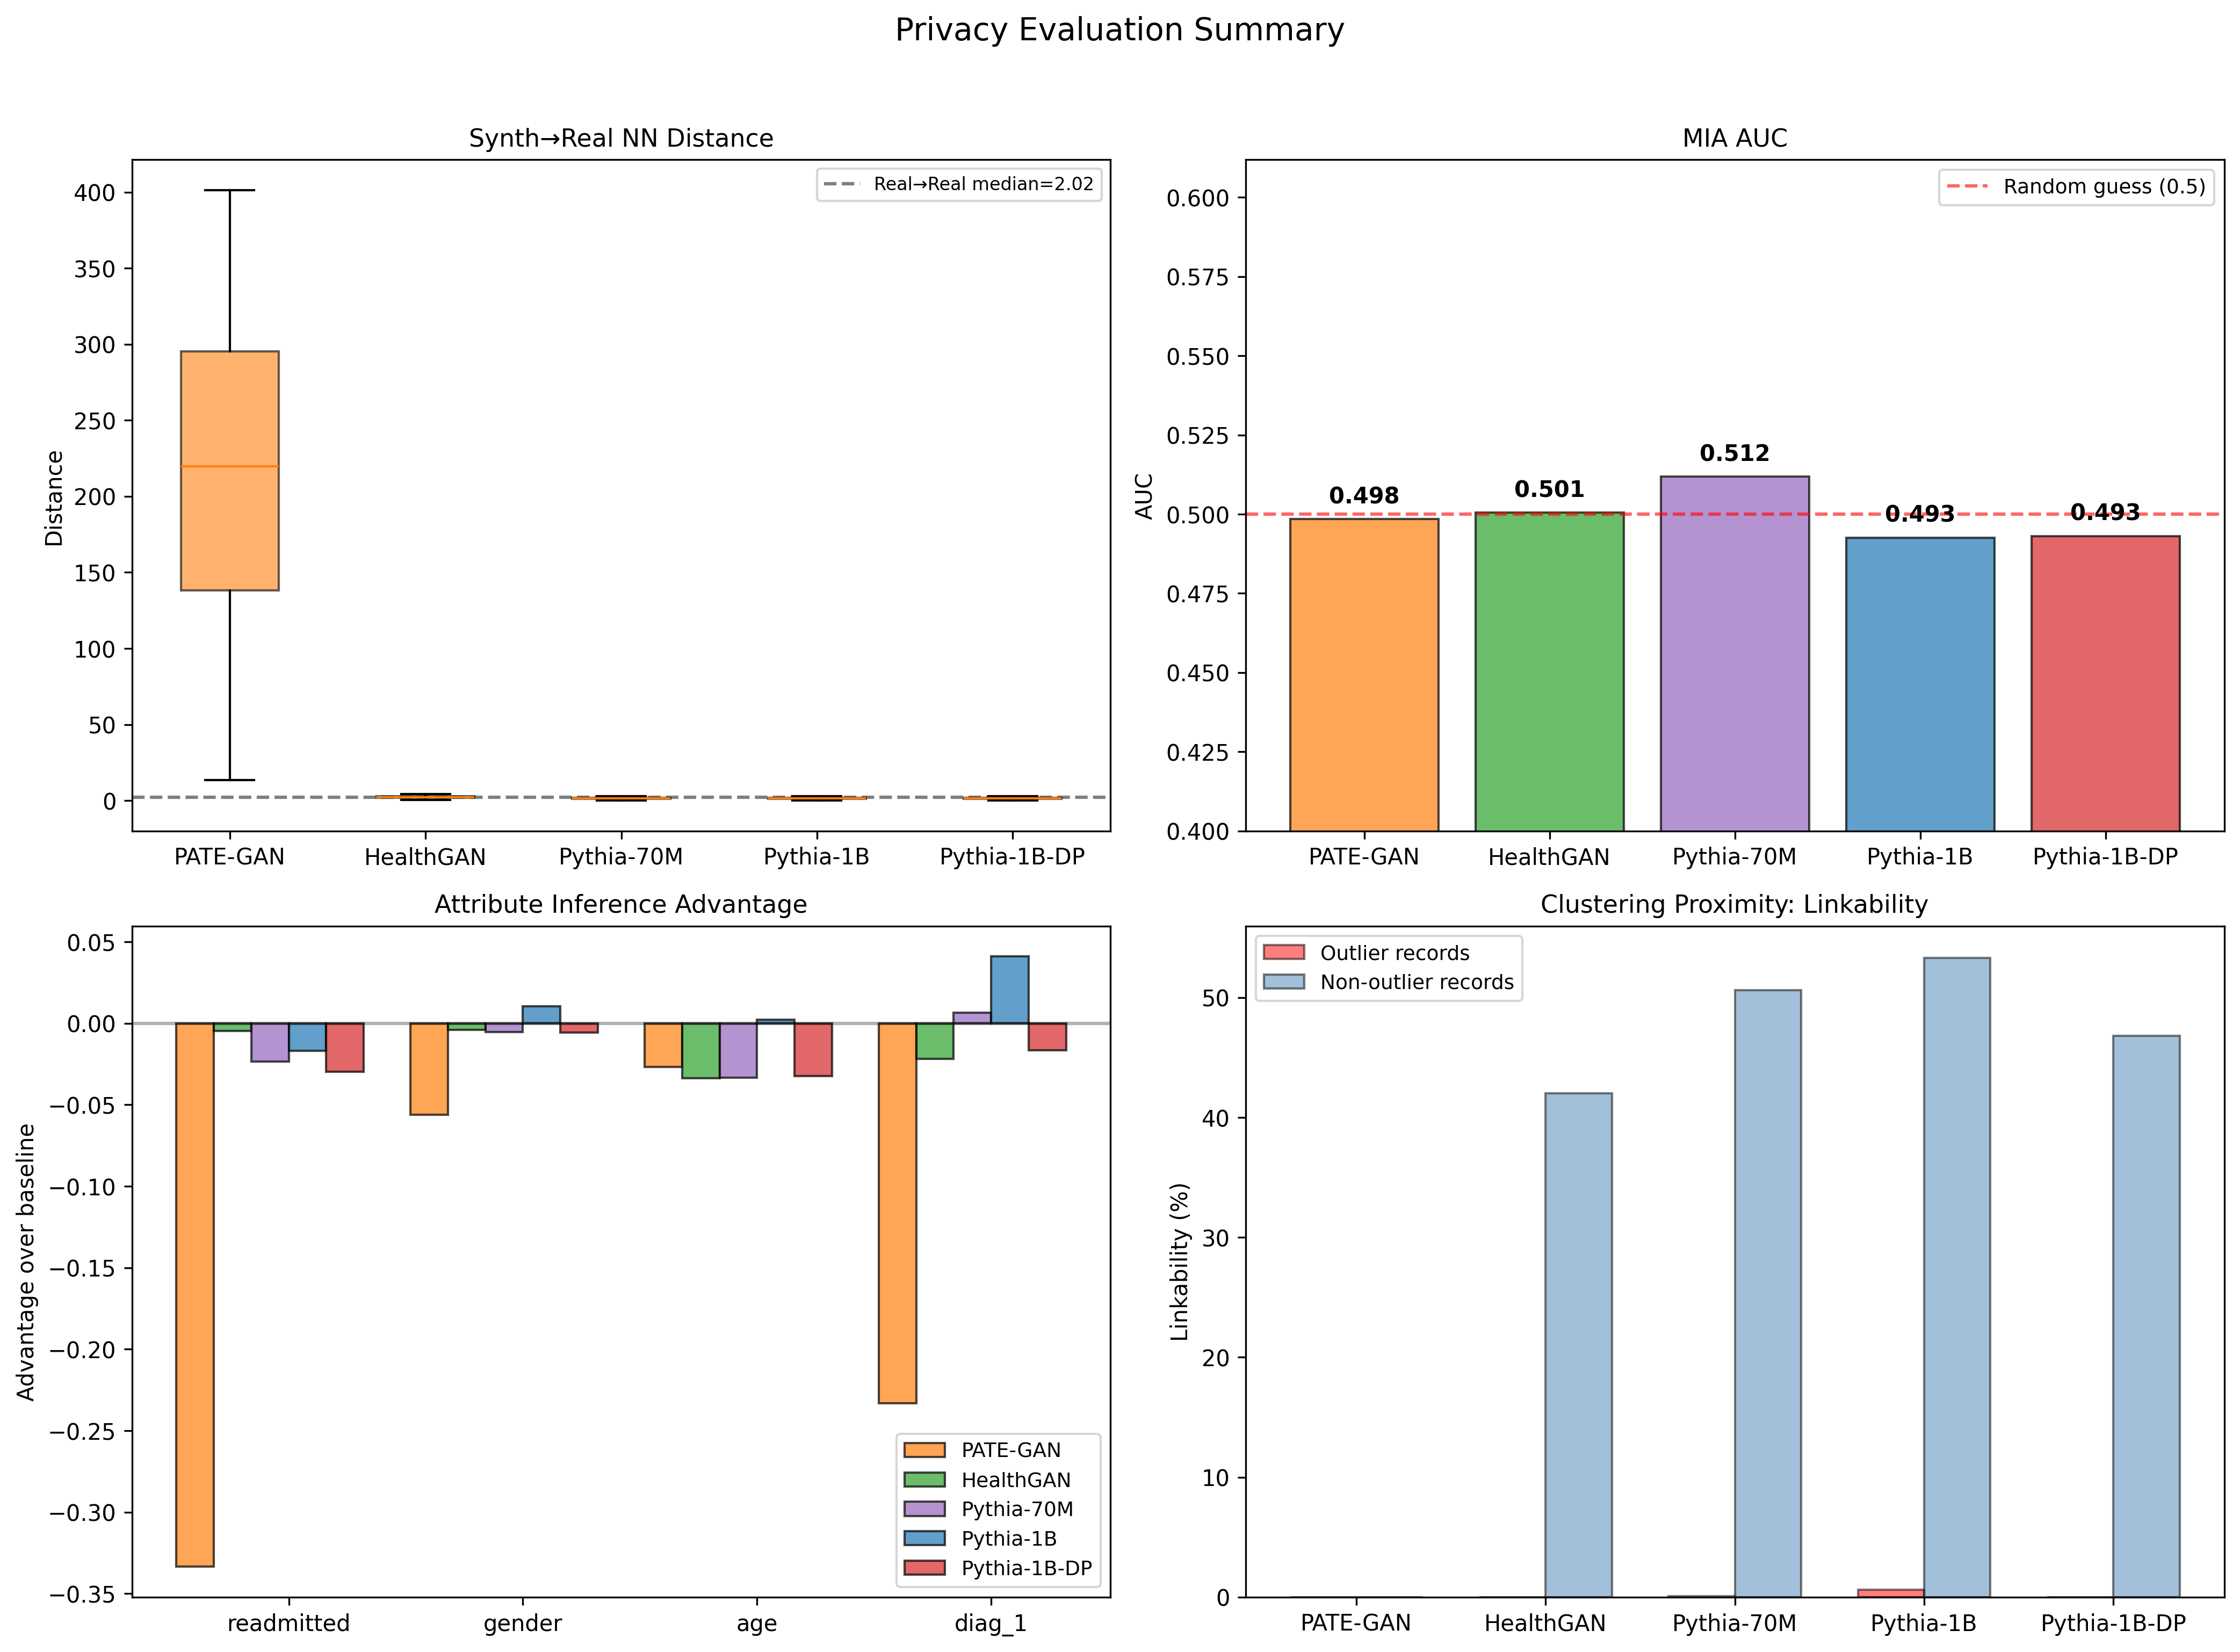
\includegraphics[width=\textwidth]{images/results/3e-privacy_evaluation}
\caption{Consolidated privacy diagnostics across the five generators:
(a)~synthetic-to-real nearest-neighbour distance on a log scale,
(b)~membership-inference AUC
against the random-guess baseline, (c)~attribute-inference
advantage per attribute, and (d)~outlier versus non-outlier
linkability.}
\label{fig:rq2:privacy}
\end{figure}

\subsection{Comparative Aggregation Results}
\label{sec:results:rq2:aggregation}

The per-metric utility and privacy results of the two preceding
subsections are now combined into the small set of aggregation views
introduced in Section~\ref{sec:eval:aggregate}. These views are
interpretive rather than decisive. The comparative claims remain grounded
in the raw metric values, and the presentation proceeds from the unscaled
summary table to the scaled visual displays. The comprehensive table is
therefore given first as the numerical reference, followed by the
privacy-utility landscape, the utility radar, the utility-privacy
heatmap, and finally the Pareto analysis that addresses the balance
question of RQ2.

\paragraph{Comprehensive Summary:}
\label{sec:results:rq2:table}

Table~\ref{tab:rq2:summary} collects the twelve headline single-number
metrics for the five generators and the real reference in a single view,
grouped by pillar and branch. It preserves the raw values used for the
main scalar comparison. Feature-importance agreement is reported in the
predictive-utility subsection and included in the utility radar, but is
not repeated here so that the table remains aligned with the twelve
headline rows defined in the methodology. The best value per row among
the synthetic generators is shown in bold for the utility rows. The
privacy rows are left unmarked because PATE-GAN's distance metrics, as
noted, reflect collapse rather than protection.

\begin{table}[H]
\centering
\footnotesize
\setlength{\tabcolsep}{3.5pt}
\caption{Comprehensive summary of the twelve headline metrics across the
five generators and the real (TRTR) reference. Arrows indicate the
preferred direction; ($\approx 0.5$) indicates that values closest to
$0.5$ are best, and ($\approx 0$) indicates negligible leakage.The nearest-neighbour distance and its normalised ratio should be
interpreted relative to the real-data reference values of
$\approx 2.02$ and $\approx 1$, respectively. Lower values indicate
increased proximity risk. Higher values suggest greater separation only
when the synthetic data remain consistent with the real-data
distribution. Otherwise, they may indicate poor fidelity rather than
stronger privacy. Bold marks the best synthetic value on each utility row.
PATE-GAN's nearest-neighbour distance and ratio are not treated as
protective because they reflect off-manifold output and should be read
with Section~\ref{sec:results:rq2:privacy}.}
\label{tab:rq2:summary}
% Auto-generated by data_analysis.ipynb (4c). Do not edit by hand.
% Requires booktabs.
\begin{tabular}{lcccccc}
\toprule
Metric & Real & PATE-GAN & HealthGAN & Pythia-70M & Pythia-1B & Pythia-1B-DP \\
\midrule
\multicolumn{7}{l}{\emph{Statistical similarity}}\\
Mean KS $\downarrow$ & --- & 0.5381 & \textbf{0.0480} & 0.0856 & 0.0805 & 0.0992 \\
Corr.\ diff.\ $\downarrow$ & --- & 0.1142 & 0.0336 & 0.0308 & \textbf{0.0206} & 0.0466 \\
\midrule
\multicolumn{7}{l}{\emph{Predictive utility}}\\
AUC-ROC $\uparrow$ & 0.7008 & 0.5108 & 0.6312 & 0.6634 & \textbf{0.6818} & 0.5827 \\
F1 $\uparrow$ & 0.3668 & 0.0093 & 0.3824 & 0.5005 & \textbf{0.5036} & 0.2714 \\
Cox CI overlap $\uparrow$ & --- & 0.0000 & \textbf{0.5833} & 0.3077 & 0.5385 & 0.5385 \\
\midrule
\multicolumn{7}{l}{\emph{Privacy}}\\
NN dist.\ median $\uparrow$ & --- & 219.879 & 2.233 & 1.440 & 1.406 & 1.533 \\
NNDR median $\uparrow$ & --- & 104.601 & 1.063 & 0.721 & 0.698 & 0.763 \\
MIA AUC ($\approx 0.5$) & --- & 0.4984 & 0.5005 & 0.5119 & 0.4926 & 0.4931 \\
MIA advantage $\downarrow$ & --- & $-0.0016$ & 0.0005 & 0.0119 & $-0.0074$ & $-0.0069$ \\
NNAA priv.\ loss ($\approx 0$) & --- & $-0.0001$ & 0.0017 & 0.0030 & $-0.0003$ & 0.0076 \\
Max.\ attr.\ adv.\ $\downarrow$ & --- & $-0.0266$ & $-0.0040$ & 0.0064 & 0.0410 & $-0.0056$ \\
Outlier link.\ \% $\downarrow$ & --- & 0.0 & 0.0 & 0.1 & 0.6 & 0.0 \\
\bottomrule
\end{tabular}

\end{table}

The table makes the division of strengths explicit. On the utility side,
Pythia-1B is strongest on correlation difference, AUC-ROC, and F1, while
HealthGAN is strongest on mean KS and Cox confidence-interval overlap.
The table therefore separates predictive and joint-structure performance
from marginal and survival-model agreement, rather than identifying one
uniformly superior generator. On the privacy side, membership-inference
AUC, membership-inference advantage, and NNAA privacy loss remain close
to their baseline values for all usable generators. The remaining
separation is metric-specific. HealthGAN is the only usable generator
above the NNDR unity reference line, while Pythia-1B shows the only
positive maximum attribute-inference advantage, a signal that is not
present for Pythia-1B-DP. These differences are revisited in the
within-family DP analysis of Section~\ref{sec:results:rq3}.

\paragraph{Privacy-Utility Landscape:}
\label{sec:results:rq2:landscape}

Figure~\ref{fig:rq2:landscape} positions all five generators on a single
privacy-utility plane, with predictive utility (Gradient-Boosting TSTR
AUC-ROC) on the horizontal axis and a distance-based privacy measure (the
median nearest-neighbour distance ratio) on the vertical axis. The dashed
reference lines mark the real-data utility ceiling (AUC $0.701$) and the
NNDR reference line of unity. This is the primary figure for the first
half of RQ2 where it shows where each family sits on the selected AUC-ROC/NNDR
view.

\begin{figure}[!ht]
\centering
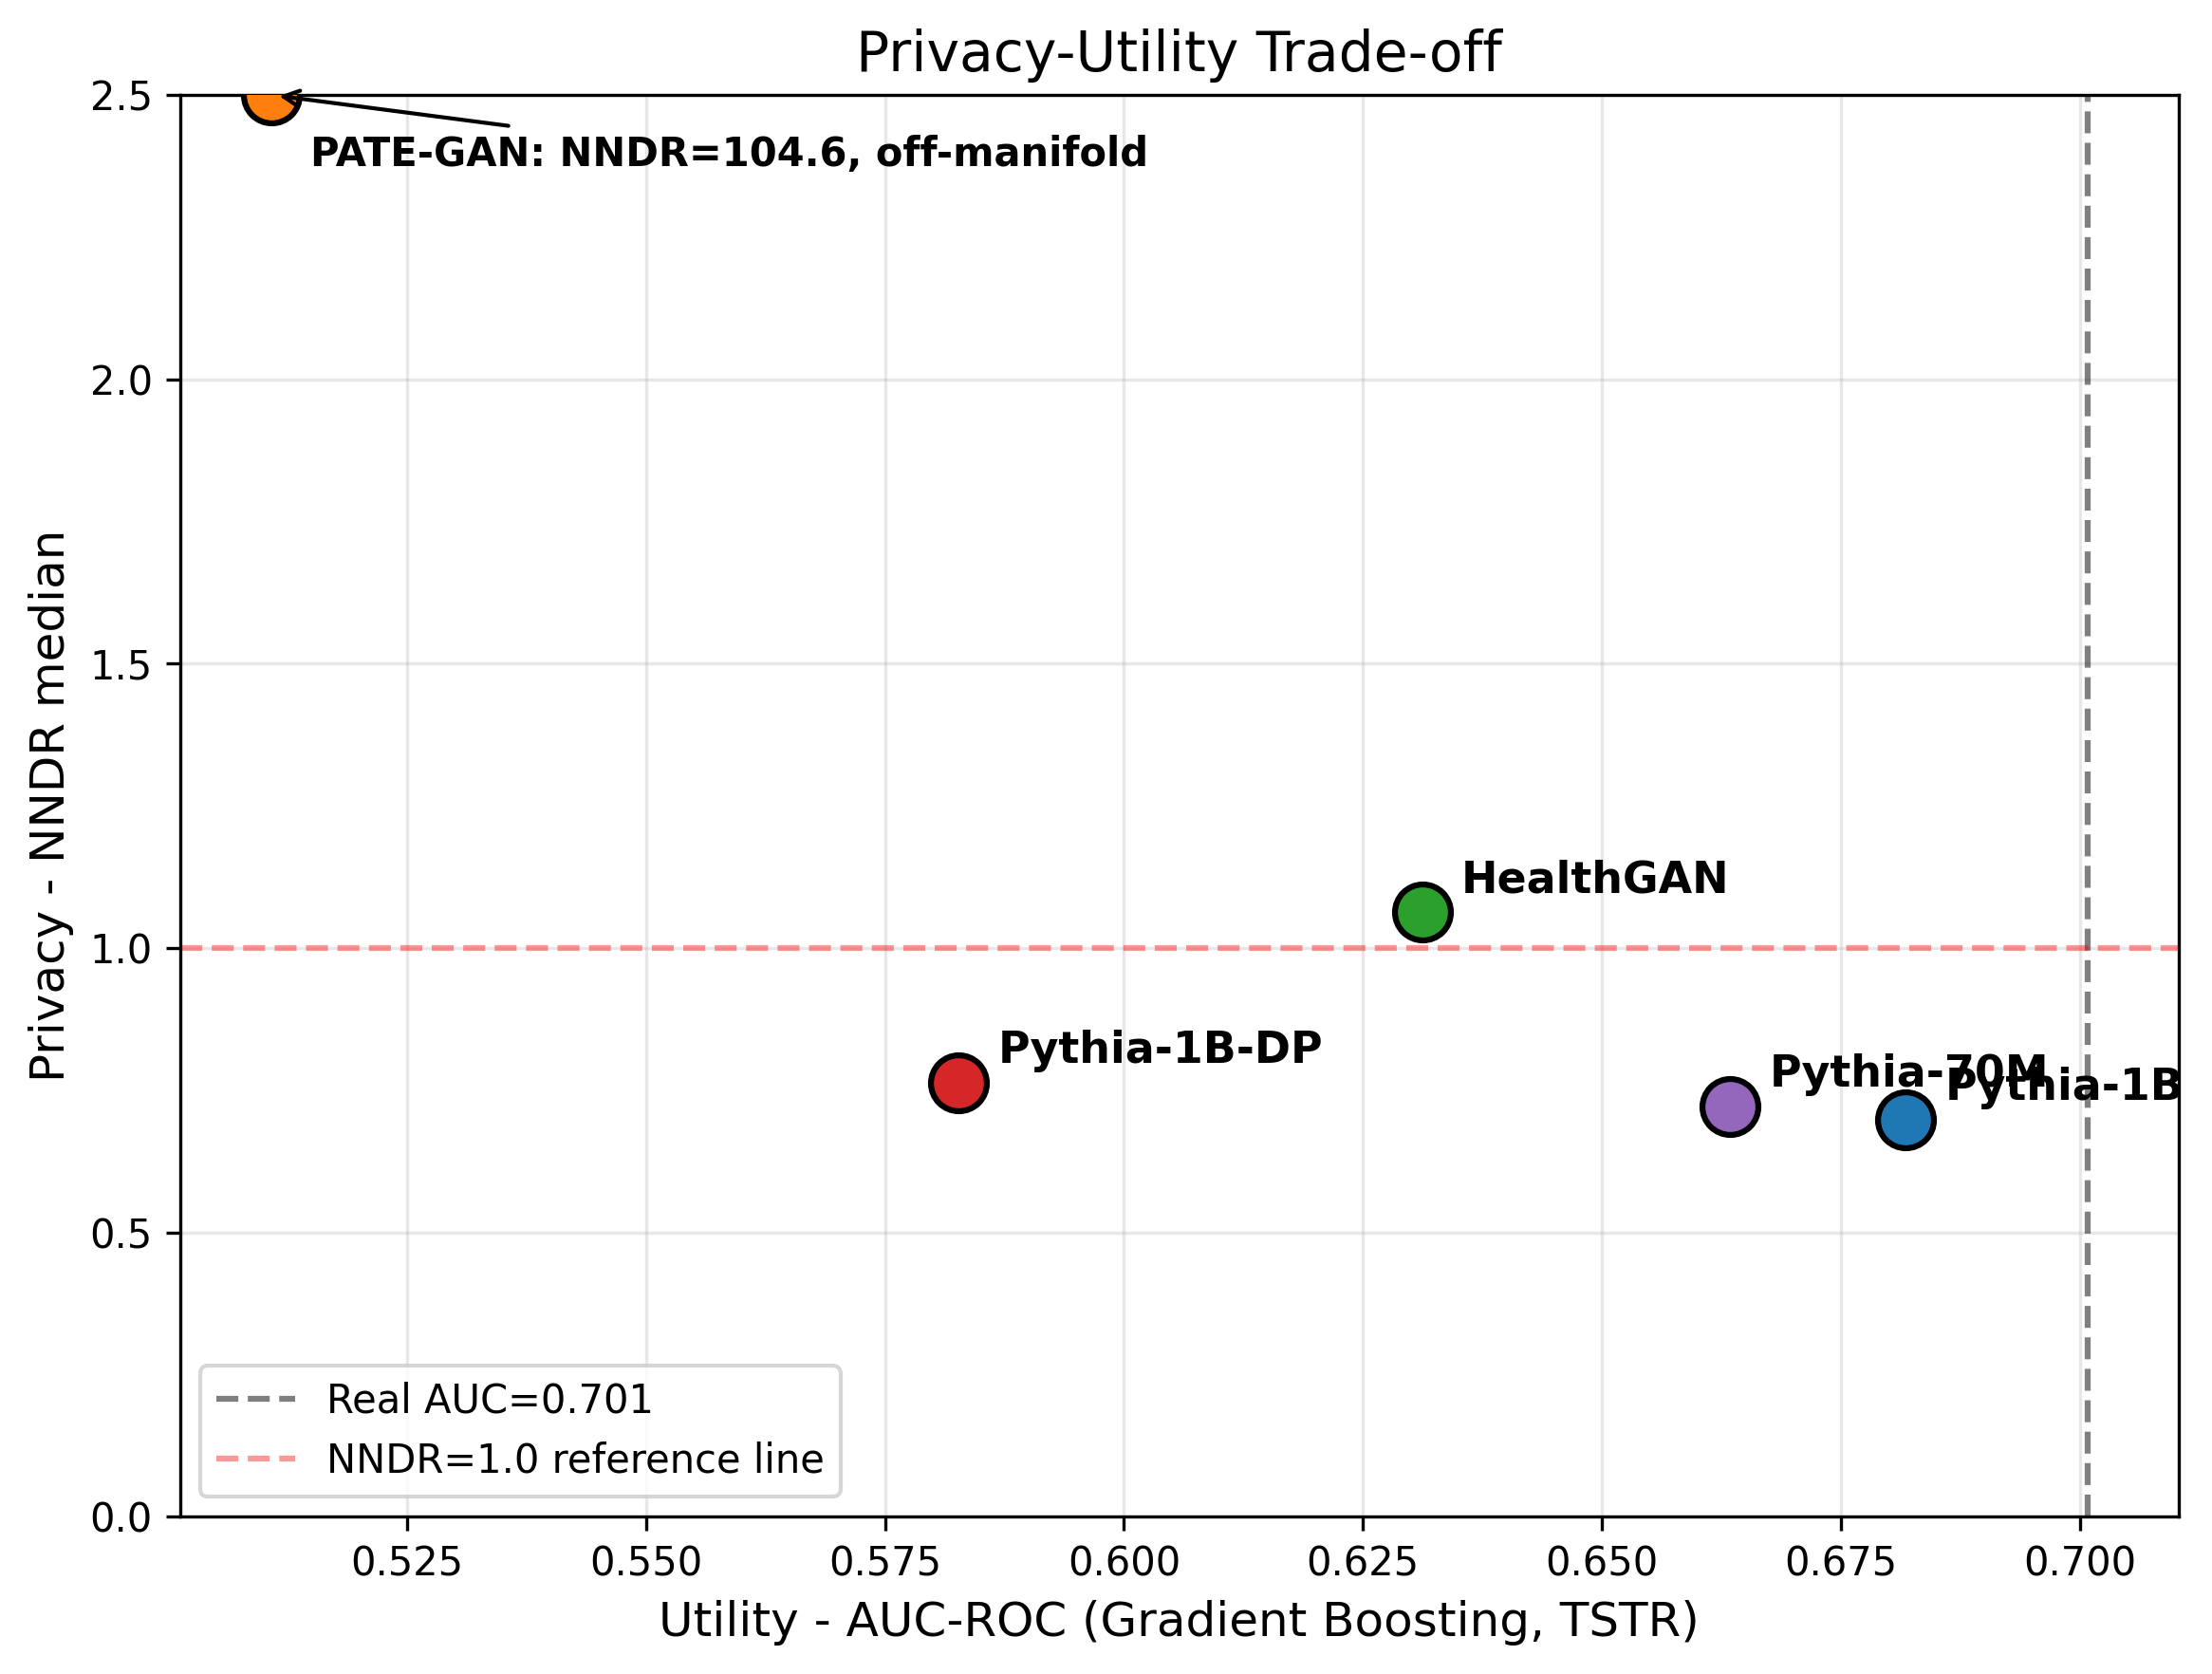
\includegraphics[width=0.85\textwidth]{images/results/4a-privacy_utility_landscape}
\caption{Privacy-utility landscape across the five generators. The
horizontal axis reports predictive utility (Gradient-Boosting TSTR
AUC-ROC), and the vertical axis reports median NNDR, where values above
$1.0$ indicate that the median synthetic-to-real distance is not below the
real-to-real reference scale. For readability, the PATE-GAN marker is shown
at a capped y-position. True median NNDR is $104.6$, as indicated by
the annotation. This inflated value reflects off-manifold output rather
than usable privacy protection. PATE-GAN is included for landscape
completeness and interpreted as the GAN family's DP-enforced operating
point (\S\ref{sec:discussion:limit:pategan-dual-role}).}
\label{fig:rq2:landscape}
\end{figure}

The plane separates into two regimes. PATE-GAN occupies an isolated
position high on the privacy axis (NNDR $\approx 105$) but at the lowest
utility (AUC $0.511$). As established in
Section~\ref{sec:results:rq2:privacy}, its extreme distance ratio is an
artefact of distributional collapse rather than genuine protection. The
remaining four generators lie close together near the NNDR unity reference
line and spread along the utility axis: Pythia-1B-DP at the low-utility end (AUC
$0.583$), then HealthGAN ($0.631$), Pythia-70M ($0.663$), and Pythia-1B
($0.682$) closest to the real-data ceiling. Among these usable
generators, HealthGAN alone sits at or above the NNDR unity reference line
(NNDR $1.063$), while the three Pythia variants fall just below it (NNDR
$0.70$-$0.76$). No single family dominates this selected two-axis plane.
LLM family supplies the highest-utility operating points, whereas
GAN family supplies the only usable point above the NNDR unity reference
line.

\paragraph{Utility Radar Comparison:}
\label{sec:results:rq2:radar}

Figure~\ref{fig:rq2:radar} overlays the five generators across six
normalised utility axes: AUC-ROC, F1, marginal fidelity ($1-$mean KS),
correlation preservation ($1-$CorrDiff), Cox confidence-interval overlap,
and feature-importance agreement. Each axis is min-max scaled to
$[0,1]$, with the real TRTR result used as a scaling anchor where
applicable but not plotted as a generator. Privacy metrics are excluded
from this radar because several privacy diagnostics have threshold-based
or two-sided interpretations and are therefore less suitable for a single
``larger is better'' radial display.

\begin{figure}[H]
\centering
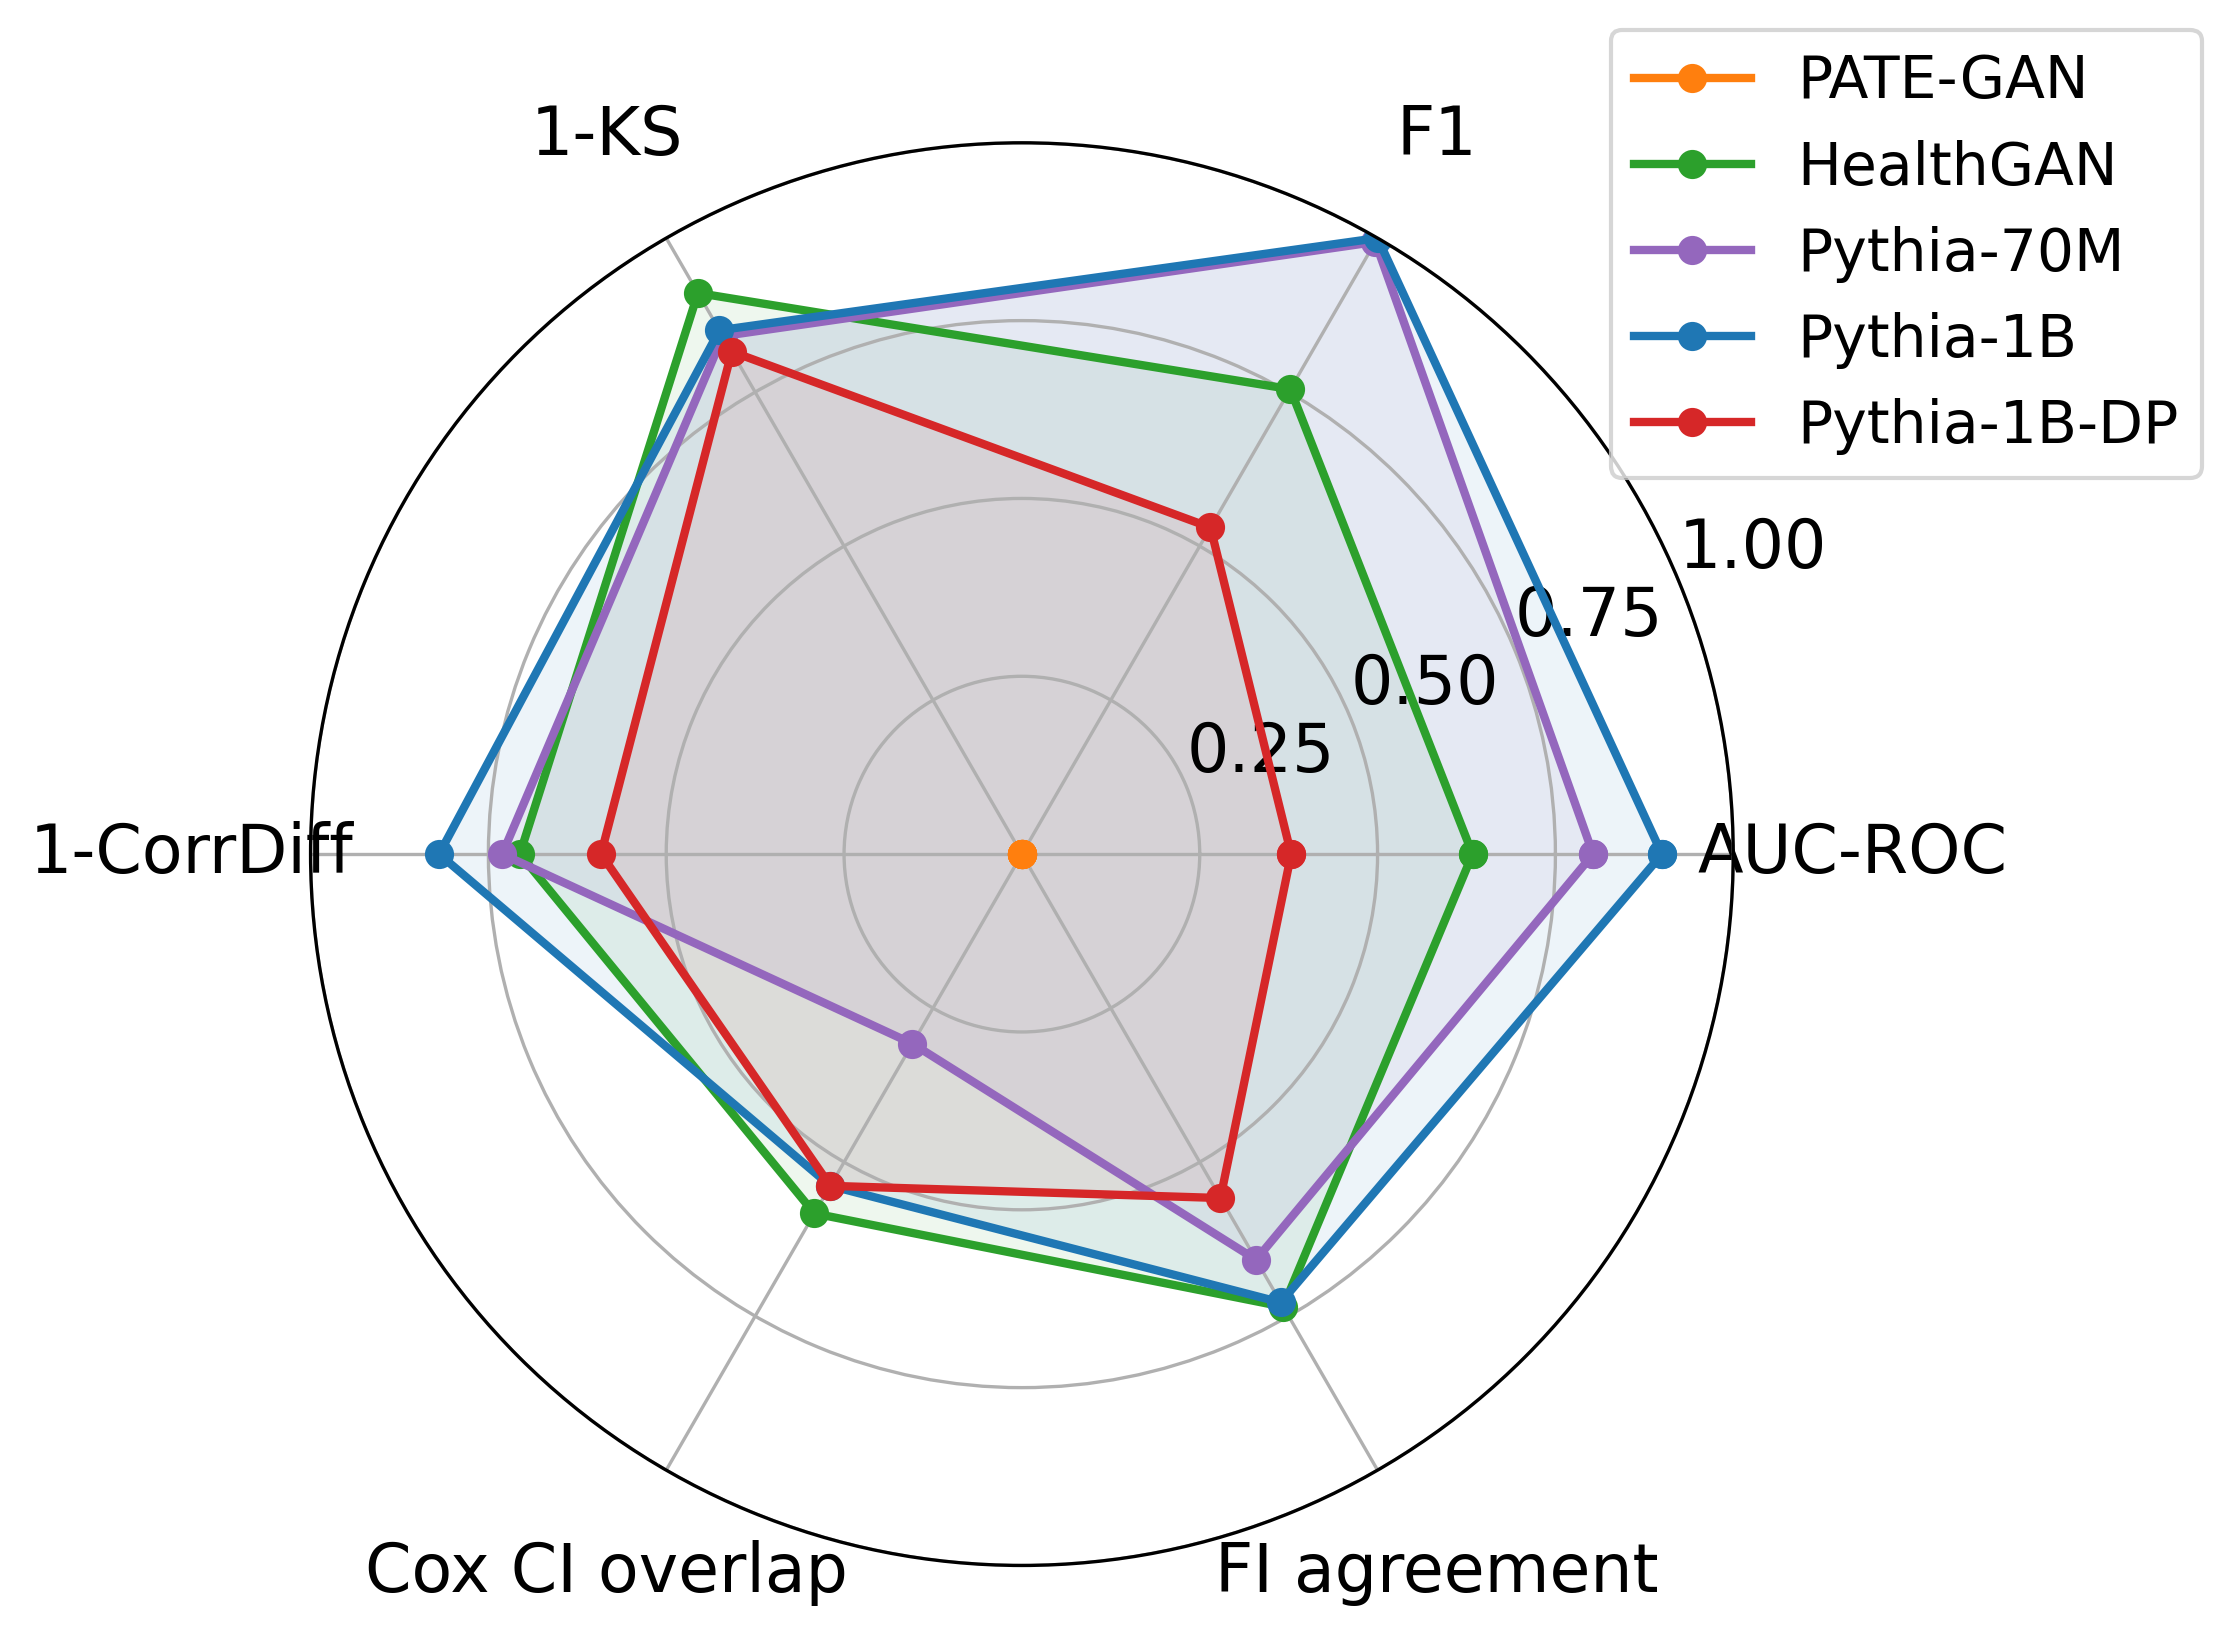
\includegraphics[width=0.78\textwidth]{images/results/4b-utility_radar}
\caption{Utility Radar Comparison across six min-max scaled utility axes:
AUC-ROC, F1, $1-$KS, $1-$CorrDiff, Cox confidence-interval overlap, and
feature-importance agreement. Larger radius indicates stronger relative
utility on the plotted axis.}
\label{fig:rq2:radar}
\end{figure}

The radar should be interpreted as a qualitative profile view rather than a scalar ranking.
The main advantage is, differently scaled utility measures can be
inspected on a common visual scale. It makes broad and narrow utility
profiles easier to compare. The limitation of this evaluation is that min-max scaling is
relative to the models included in the figure and does not preserve the
absolute distances of the original metrics. The polygon area should
therefore not be read as a formal performance score.

The pattern is consistent with the preceding utility results. PATE-GAN
sits at the centre because it is the lowest of the five generators on every
utility axis, which min-max scaling maps to zero. This is a relative floor
rather than zero utility, and the underlying values (for example TSTR
AUC-ROC $0.511$) are reported in Table~\ref{tab:rq2:summary}. Its central
position reflects weak predictive transfer, poor correlation preservation,
and the absence of Cox confidence-interval overlap. The non-collapsed generators form broader
profiles. Pythia-1B has the strongest relative profile on AUC-ROC, F1,
and correlation preservation, with high feature-importance agreement.
HealthGAN has the strongest relative marginal fidelity and Cox
confidence-interval overlap. Pythia-1B-DP remains non-collapsed but is
lower than Pythia-1B on the two predictive axes, which is consistent with
the TSTR utility cost reported above.

\paragraph{Utility-Privacy Heatmap:}
\label{sec:results:rq2:heatmap}

Figure~\ref{fig:rq2:heatmap} provides the metric-level inspection view
defined in Section~\ref{sec:eval:aggregate:heatmap}. Each metric is
min-max scaled to $[0,1]$ across the generators. The orientation
of the two blocks are different. Utility metrics are shown as performance, so a larger
value is better. Privacy metrics are shown as risk, so a larger
value is worse. Here only the leakage side of the middle-ideal privacy
metrics counted. The display
therefore exposes the full per-metric pattern without collapsing the
metrics into a single composite score.

\begin{figure}[H]
\centering
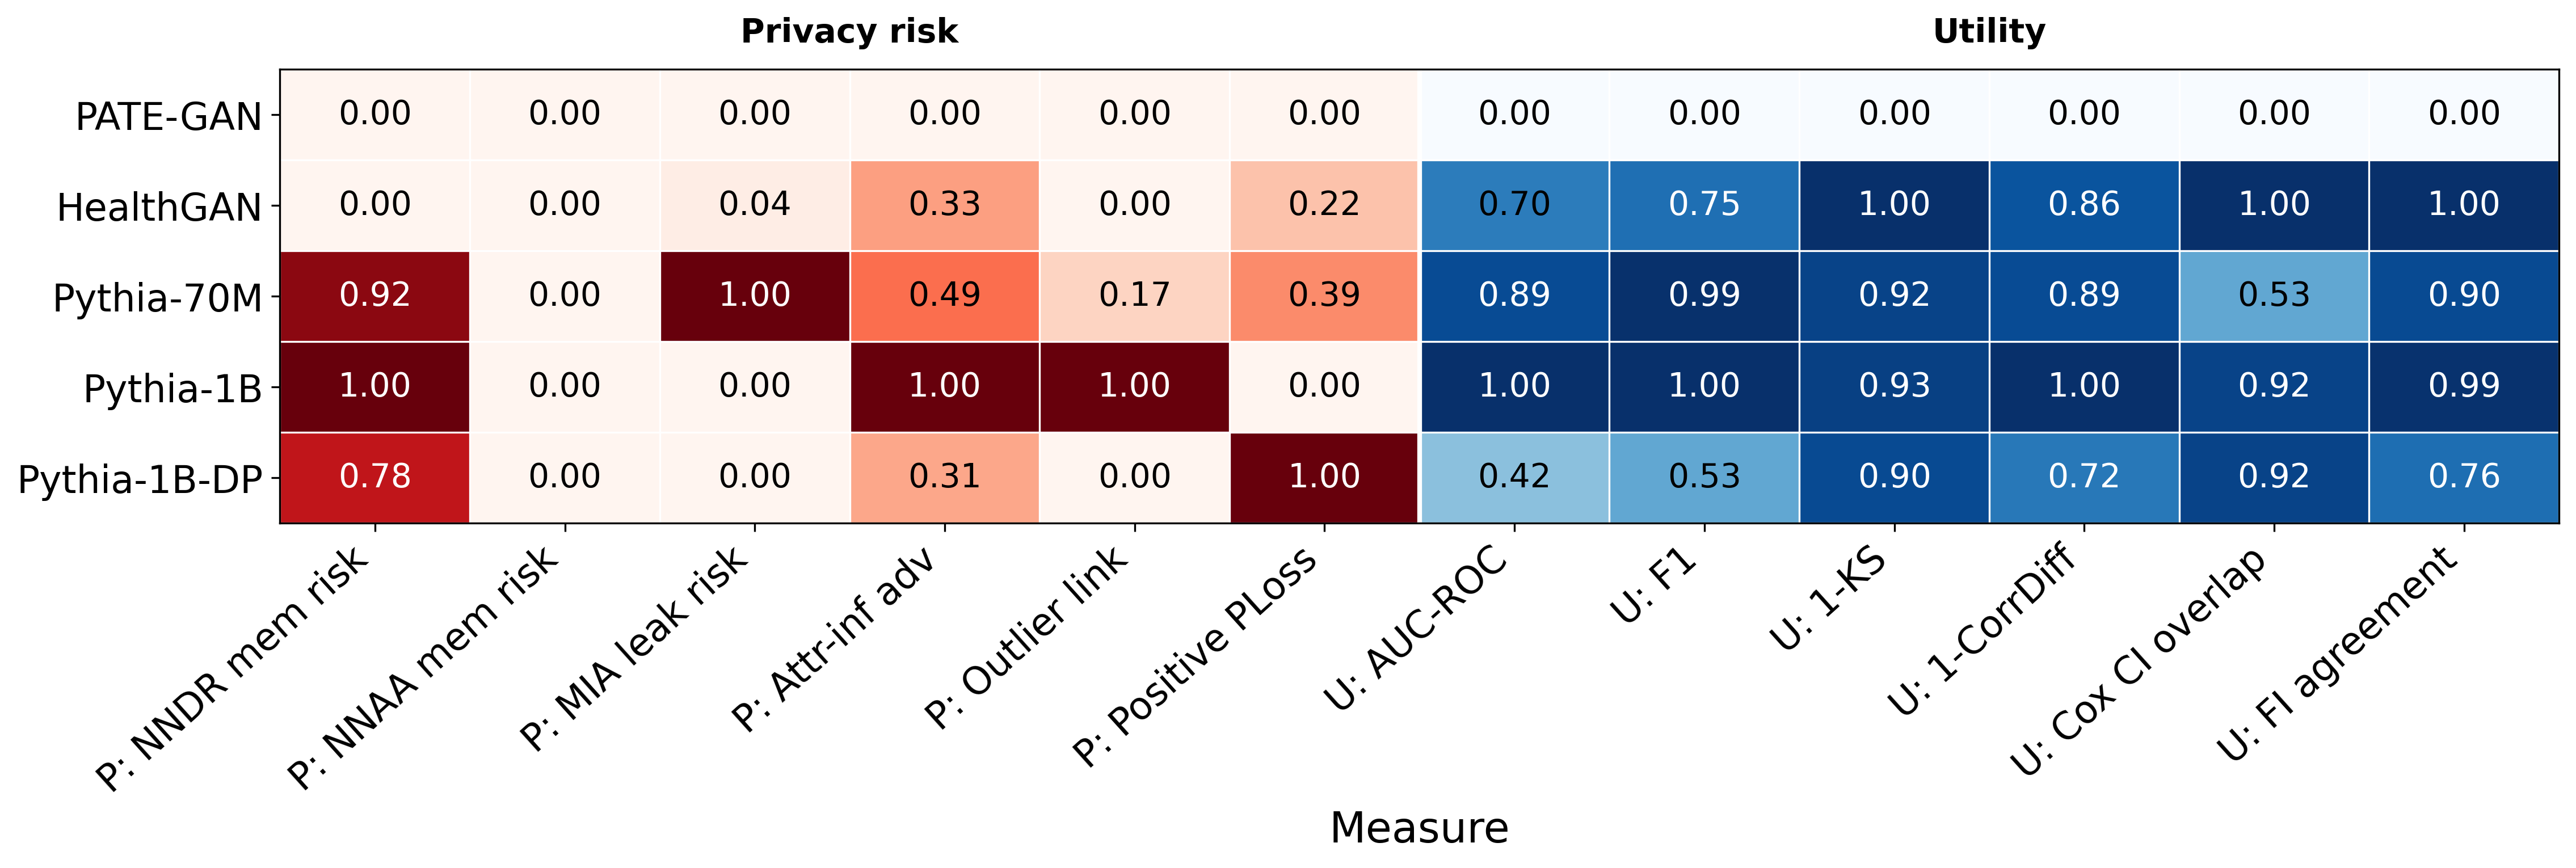
\includegraphics[width=0.90\textwidth]{images/results/4e-utility_privacy_heatmap}
\caption{Utility-privacy heatmap across the five generators. Utility
metrics are oriented as performance and privacy metrics as risk, each
min-max scaled to $[0,1]$ across the generators. Darker cells indicate 
better utility but greater privacy risk. Therefore,
dark utility and pale privacy cells are preferred. Only the leakage side of
the middle-ideal privacy metrics is counted, so a distributionally
collapsed generator can appear low-risk in the privacy block and must be
read together with the summary table of Table~\ref{tab:rq2:summary}.}
\label{fig:rq2:heatmap}
\end{figure}

The heatmap confirms the patterns observed in the individual metrics.
However, because each column is min-max scaled across the generators, the
colours represent relative rather than absolute differences. On the utility
side, PATE-GAN performs substantially worse than the other four generators
across both similarity and predictive metrics.

Most privacy values are close to their reference levels
(Table~\ref{tab:rq2:summary}). So, the colour scale can make small
privacy differences appear larger than they are. The Pythia variants show
the strongest relative proximity signal because their NNDR values are
below $1.0$. Pythia-70M has the highest relative membership-inference
signal, while Pythia-1B has the highest attribute-inference and outlier-
linkability signals. These signals are reduced or absent in Pythia-1B-DP.

PATE-GAN appears pale in the privacy block because its records are far from
the real-data distribution, not because it provides stronger practical
privacy. A pale cell therefore indicates low utility in the utility block
but low apparent risk in the privacy block. The heatmap should
be interpreted as a relative comparison and read together with the raw
values in Table~\ref{tab:rq2:summary}.

\paragraph{Pareto Analysis:}
\label{sec:results:rq2:pareto}

To examine the privacy and utility balance in RQ2, Pareto analysis is
applied to the two axes shown in Figure~\ref{fig:rq2:landscape}.
Gradient-Boosting TSTR AUC-ROC represents utility, while median NNDR
represents privacy. The analysis follows the rule defined in
Section~\ref{sec:eval:aggregate:tradeoff}. A generator is Pareto-optimal
when no other generator performs at least as well on both axes and better
on one.

Using all five generators, the Pareto frontier includes PATE-GAN,
HealthGAN, Pythia-70M, and Pythia-1B. Pythia-1B-DP is the only dominated
generator because HealthGAN achieves higher utility ($0.631$ versus
$0.583$) and a higher NNDR ($1.063$ versus $0.763$). PATE-GAN appears on
the frontier only because its output produces an extremely high NNDR. Its
output differs greatly from the real-data distribution, so it is not
considered a usable solution. After excluding PATE-GAN, the usable
frontier contains HealthGAN, Pythia-70M, and Pythia-1B. The two
non-private LLMs provide higher utility, while HealthGAN provides the
higher NNDR.

The dominance of Pythia-1B-DP applies only to this AUC-ROC and NNDR
comparison. NNDR does not capture all forms of privacy protection,
including the reduction in attribute-inference leakage achieved by
Pythia-1B-DP
(Section~\ref{sec:results:rq2:privacy:aia}). Therefore, this result does
not show that differential privacy is generally ineffective. Its broader
costs and benefits are examined in Section~\ref{sec:results:rq3}.

\subsection*{Findings for Research Question 2}
\label{sec:results:rq2:answer}

RQ2 does not identify one universally superior generator family. Instead,
the evaluated configurations occupied different positions in the
privacy-utility trade-off. The non-private Pythia models provided the
strongest downstream predictive utility and pairwise linear-dependency
preservation, whereas HealthGAN provided the strongest marginal fidelity
and the better record-proximity profile among the usable
generators. The comparison therefore identifies different options
depending on whether the intended use prioritises statistical resemblance,
predictive performance, or empirical privacy risk.

Pythia-1B achieved the highest Gradient-Boosting TSTR
AUC-ROC ($0.6818$) and the lowest pairwise correlation difference
($0.0206$) when we are comparing on the utility side.
Pythia-70M followed with an AUC-ROC of $0.6634$ and similarly
strong downstream performance. HealthGAN achieved a lower AUC-ROC
($0.6312$) but produced the best marginal-distribution fidelity with a
mean KS statistic of $0.0480$. It also achieved the highest
feature-importance agreement ($0.914$). Although Pythia-1B was practically
similar at $0.911$. HealthGAN additionally had highest Cox
confidence-interval overlap. However, because the fitted duration was
time in hospital rather than time to readmission, this result is treated
only as a model-specific association diagnostic and not as clinical
survival evidence.

The selected privacy metrics separated the usable generators less clearly.
Membership-inference AUC remained close to $0.5$, and NNAA privacy loss
remained close to zero across all configurations. HealthGAN's median NNDR
of $1.063$ was closest to the real-data spacing reference of one. It also
showed no positive attribute-inference advantage and zero outlier
linkability. Pythia-1B had a lower NNDR of $0.698$, which indicates greater proximity
between synthetic and real records. It also had the highest observed
attribute-inference advantage of $0.0410$, mainly for the diagnosis
attribute. It had the highest outlier linkability, although the
absolute value remained low at $0.6\%$. These results do not establish
that HealthGAN is secure or that Pythia-1B is unsafe. They indicate that
Pythia-1B produced the clearest relative privacy-risk signals under the
specified attacks and linkability definition.

Pythia-70M occupied an intermediate trade-off position. Its predictive
utility was close to that of Pythia-1B, while its attribute-inference
advantage ($0.0064$) and outlier linkability ($0.1\%$) were lower.
The model therefore remained non-dominated in the primary AUC-ROC-NNDR Pareto
analysis, although it did not lead either predictive utility or
real-reference proximity. PATE-GAN was not considered a meaningful
privacy-utility option because its apparently favourable distances and
zero outlier linkability resulted from distributional collapse rather
than usable privacy protection.

Pythia-1B-DP represents a separate decision case. Compared with Pythia-1B,
the model reduced the maximum attribute-inference advantage from $+0.0410$ to
$-0.0056$ and outlier linkability from $0.6\%$ to zero. On the contrary, its
predictive utility decreased from $0.6818$ to $0.5827$. It is therefore relevant
when a formal differential-privacy requirement takes precedence, but it
does not provide the strongest observed predictive utility. The detailed
within-family consequences of differential privacy are addressed in
Section~\ref{sec:results:rq3}.

Overall, HealthGAN provides a more conservative balance between privacy
and utility. Pythia-1B is the preferred
option when predictive utility is the main priority and its higher
observed attribute-inference and outlier-linkability signals are
considered acceptable for the intended use and governance setting.
These recommendations are limited to the evaluated configurations,
dataset, metrics, and attacks. Because the results are based on single
point estimates without repeated-run uncertainty. Also, small numerical
differences should not be interpreted as statistically established
family-level effects.


\section{RQ3 - The Cost of DP Enforcement, Within-Family}
\label{sec:results:rq3}

% RQ3 (finalised): "At a matched privacy budget (ε=5.0), how does enforcing
% differential privacy using mechanisms appropriate to each family affect
% utility, and how do the resulting privacy-utility profiles differ
% between GAN-based (PATE-GAN vs HealthGAN) and LLM-based (Pythia 1B-DP vs
% Pythia 1B) synthesisers of tabular medical data?"
%
% The four generators analysed in this section are a subset of the five
% reported in \S\ref{sec:results:rq2}; the same experimental outputs are
% re-examined under a within-family DP-toggle lens, not re-run. Pythia-70M
% is excluded from RQ3's main comparison because DP-SGD failed at that
% scale (\S\ref{sec:results:rq3:pythia-70m-failure}).

\subsection{Convergence Failure of DP-SGD at the Pythia-70M Scale}
\label{sec:results:rq3:pythia-70m-failure}

An initial attempt to apply DP-SGD to Pythia-70M at $\varepsilon = 5.0$
failed to train usefully. The recorded training loss worsened across the
five epochs (from $3.38$ to $3.74$, peaking at $3.79$) under the
calibrated noise multiplier $\sigma = 0.436$, and the model did not
converge to a useful synthesis distribution. This suggests that the 
added noise may have weakened the useful gradient
signal at this model scale. However, gradient magnitudes were not measured
directly. The LLM-side DP comparison was therefore scaled to
Pythia-1B, which trained successfully under DP-SGD at the same privacy
budget. The finding from this is DP-SGD on small LLMs couldn't be 
applied at $\varepsilon = 5.0$. It is consistent with prior work
showing that larger LLMs tolerate DP noise more
gracefully~\cite{Li2022LargeDP}. The methodological consequence, that the
LLM-family DP toggle is operationalised at the 1B scale, is discussed in
\S\ref{sec:methods:pythia-dp:why-1b}.

\subsection{Cost of Differential Privacy on the GAN Family}
\label{sec:results:rq3:gan-toggle}

The GAN comparison examines the non-private HealthGAN and the
differentially private PATE-GAN. It shows the changes associated with
moving to a formally private GAN. However, because the models use
different architectures, these changes cannot be attributed to
differential privacy alone.
Table~\ref{tab:rq3:gan-toggle} reports the change on each headline metric.

\begin{table}[H]
\centering
\small
\caption{Within-family differential-privacy transition for the GAN family
(HealthGAN to PATE-GAN). $\Delta$ is PATE-GAN value minus 
HealthGAN value. On a utility row a negative $\Delta$ denotes a loss. 
The NNDR change should not be interpreted as a privacy improvement because
PATE-GAN's extremely high value results from its distance from the
real-data distribution. }
\label{tab:rq3:gan-toggle}
\begin{tabular}{lccc}
\toprule
Metric & HealthGAN & PATE-GAN & $\Delta$ \\
\midrule
Mean KS $\downarrow$       & 0.0480 & 0.5381 & $+0.4901$ \\
Corr.\ diff.\ $\downarrow$ & 0.0336 & 0.1142 & $+0.0806$ \\
AUC-ROC $\uparrow$         & 0.6312 & 0.5108 & $-0.1204$ \\
F1 $\uparrow$              & 0.3824 & 0.0093 & $-0.3731$ \\
Cox CI overlap $\uparrow$  & 0.5833 & 0.0000 & $-0.5833$ \\
NNDR median                & 1.063  & 104.601 & $103.538$ \\
Max.\ attr.\ adv.\ $\downarrow$ & $-0.0040$ & $-0.0266$ & $-0.0226$ \\
\bottomrule
\end{tabular}
\end{table}

Utility declines across all measures in this transition. Mean KS increases
from $0.0480$ to $0.5381$, while the correlation difference increases from
$0.0336$ to $0.1142$. AUC-ROC falls by $0.1204$ to near chance, F1
decreases from $0.3824$ to $0.0093$, and Cox confidence-interval overlap
falls from $7/12$ to $0/13$.

NNDR increases from $1.063$ to $104.601$. However, this does not represent
a genuine privacy improvement because PATE-GAN's output lies far from the
real-data distribution. The other privacy measures
change only slightly because both generators show low membership and
attribute-inference risks.

This is not a controlled comparison of differential privacy because
HealthGAN and PATE-GAN use different architectures. Therefore, the
observed utility loss cannot be attributed to differential privacy alone
(Section~\ref{sec:discussion:limit:gan-toggle-asymmetry}).

\subsection{Cost of Differential Privacy on the LLM Family}
\label{sec:results:rq3:llm-toggle}

The LLM-family comparison contrasts the non-private Pythia-1B with the
differentially private Pythia-1B-DP. Because both variants share the same
Pythia-1B backbone, the same row-as-text serialisation, and the same
low-rank fine-tuning configuration. This comparison is a
differential-privacy toggle. The only material difference is the DP-SGD
training procedure and some fine tuning parameters to accommodate DP-SGD. The private
variant was trained under a privacy budget that the accounting reports as
an achieved $\varepsilon = 4.998$ against a target of $5.0$ (with
$\delta = 10^{-5}$, gradient-clipping norm $1.0$, noise multiplier
$0.789$, and an effective batch size of $512$).
Table~\ref{tab:rq3:llm-toggle} reports the change on each headline metric.

\begin{table}[H]
\centering
\small
\caption{Within-family differential-privacy transition for the LLM family
(Pythia-1B to Pythia-1B-DP), a toggle on a shared backbone at
achieved $\varepsilon = 4.998$. $\Delta$ is the private value minus the
non-private value.}
\label{tab:rq3:llm-toggle}
\begin{tabular}{lccc}
\toprule
Metric & Pythia-1B & Pythia-1B-DP & $\Delta$ \\
\midrule
Mean KS $\downarrow$       & 0.0805 & 0.0992 & $+0.0187$ \\
Corr.\ diff.\ $\downarrow$ & 0.0206 & 0.0466 & $+0.0260$ \\
AUC-ROC $\uparrow$         & 0.6818 & 0.5827 & $-0.0991$ \\
F1 $\uparrow$              & 0.5036 & 0.2714 & $-0.2322$ \\
Cox CI overlap $\uparrow$  & 0.5385 & 0.5385 & $\phantom{+}0.0000$ \\
NNDR median                & 0.698  & 0.763  & $+0.065$ \\
Max.\ attr.\ adv.\ $\downarrow$ & $+0.0410$ & $-0.0056$ & $-0.0466$ \\
Outlier link.\ \% $\downarrow$  & 0.6 & 0.0 & $-0.6$ \\
\bottomrule
\end{tabular}
\end{table}

The cost is real and falls almost entirely on the predictive branch, where
it is uneven. AUC-ROC drops by a moderate $0.0991$ (to $0.5827$, still well
above chance), whereas F1 falls more steeply from $0.5036$ to $0.2714$,
close to a halving. The statistical-similarity branch
is barely affected (mean KS rises by only $0.0187$ and the correlation
difference by $0.0260$, both leaving the private variant comfortably within
the regime), and the survival model is untouched, with identical
confidence-interval overlap ($7/13$) before and after. On the privacy side
the toggle produces a small genuine benefit. The attribute-inference signal 
observed for primary diagnosis in the
non-private model was no longer detected under private training. The
maximum observed advantage decreased from $+0.0410$ to $-0.0056$, while
outlier linkability decreased to zero. Differential
Private training reduced predictive utility within the LLM family. The
reduction was moderate for AUC-ROC but larger for F1. However, it also
reduced the observed attribute-disclosure risk while broadly preserving
distributional fidelity and Cox-model agreement.

\subsection{Cross-Family Comparison of Differential-Privacy Cost}
\label{sec:results:rq3:arrow-plot}

Figure~\ref{fig:rq3:arrow} places the four generators on the
privacy-utility plane of Figure~\ref{fig:rq2:landscape} and draws each
within-family differential-privacy transition as an arrow from the
non-private to the private variant. The vertical axis (NNDR) is shown on a
logarithmic scale so that both transitions are visible despite PATE-GAN's
off-scale distance ratio.

\begin{figure}[!htbp]
\centering
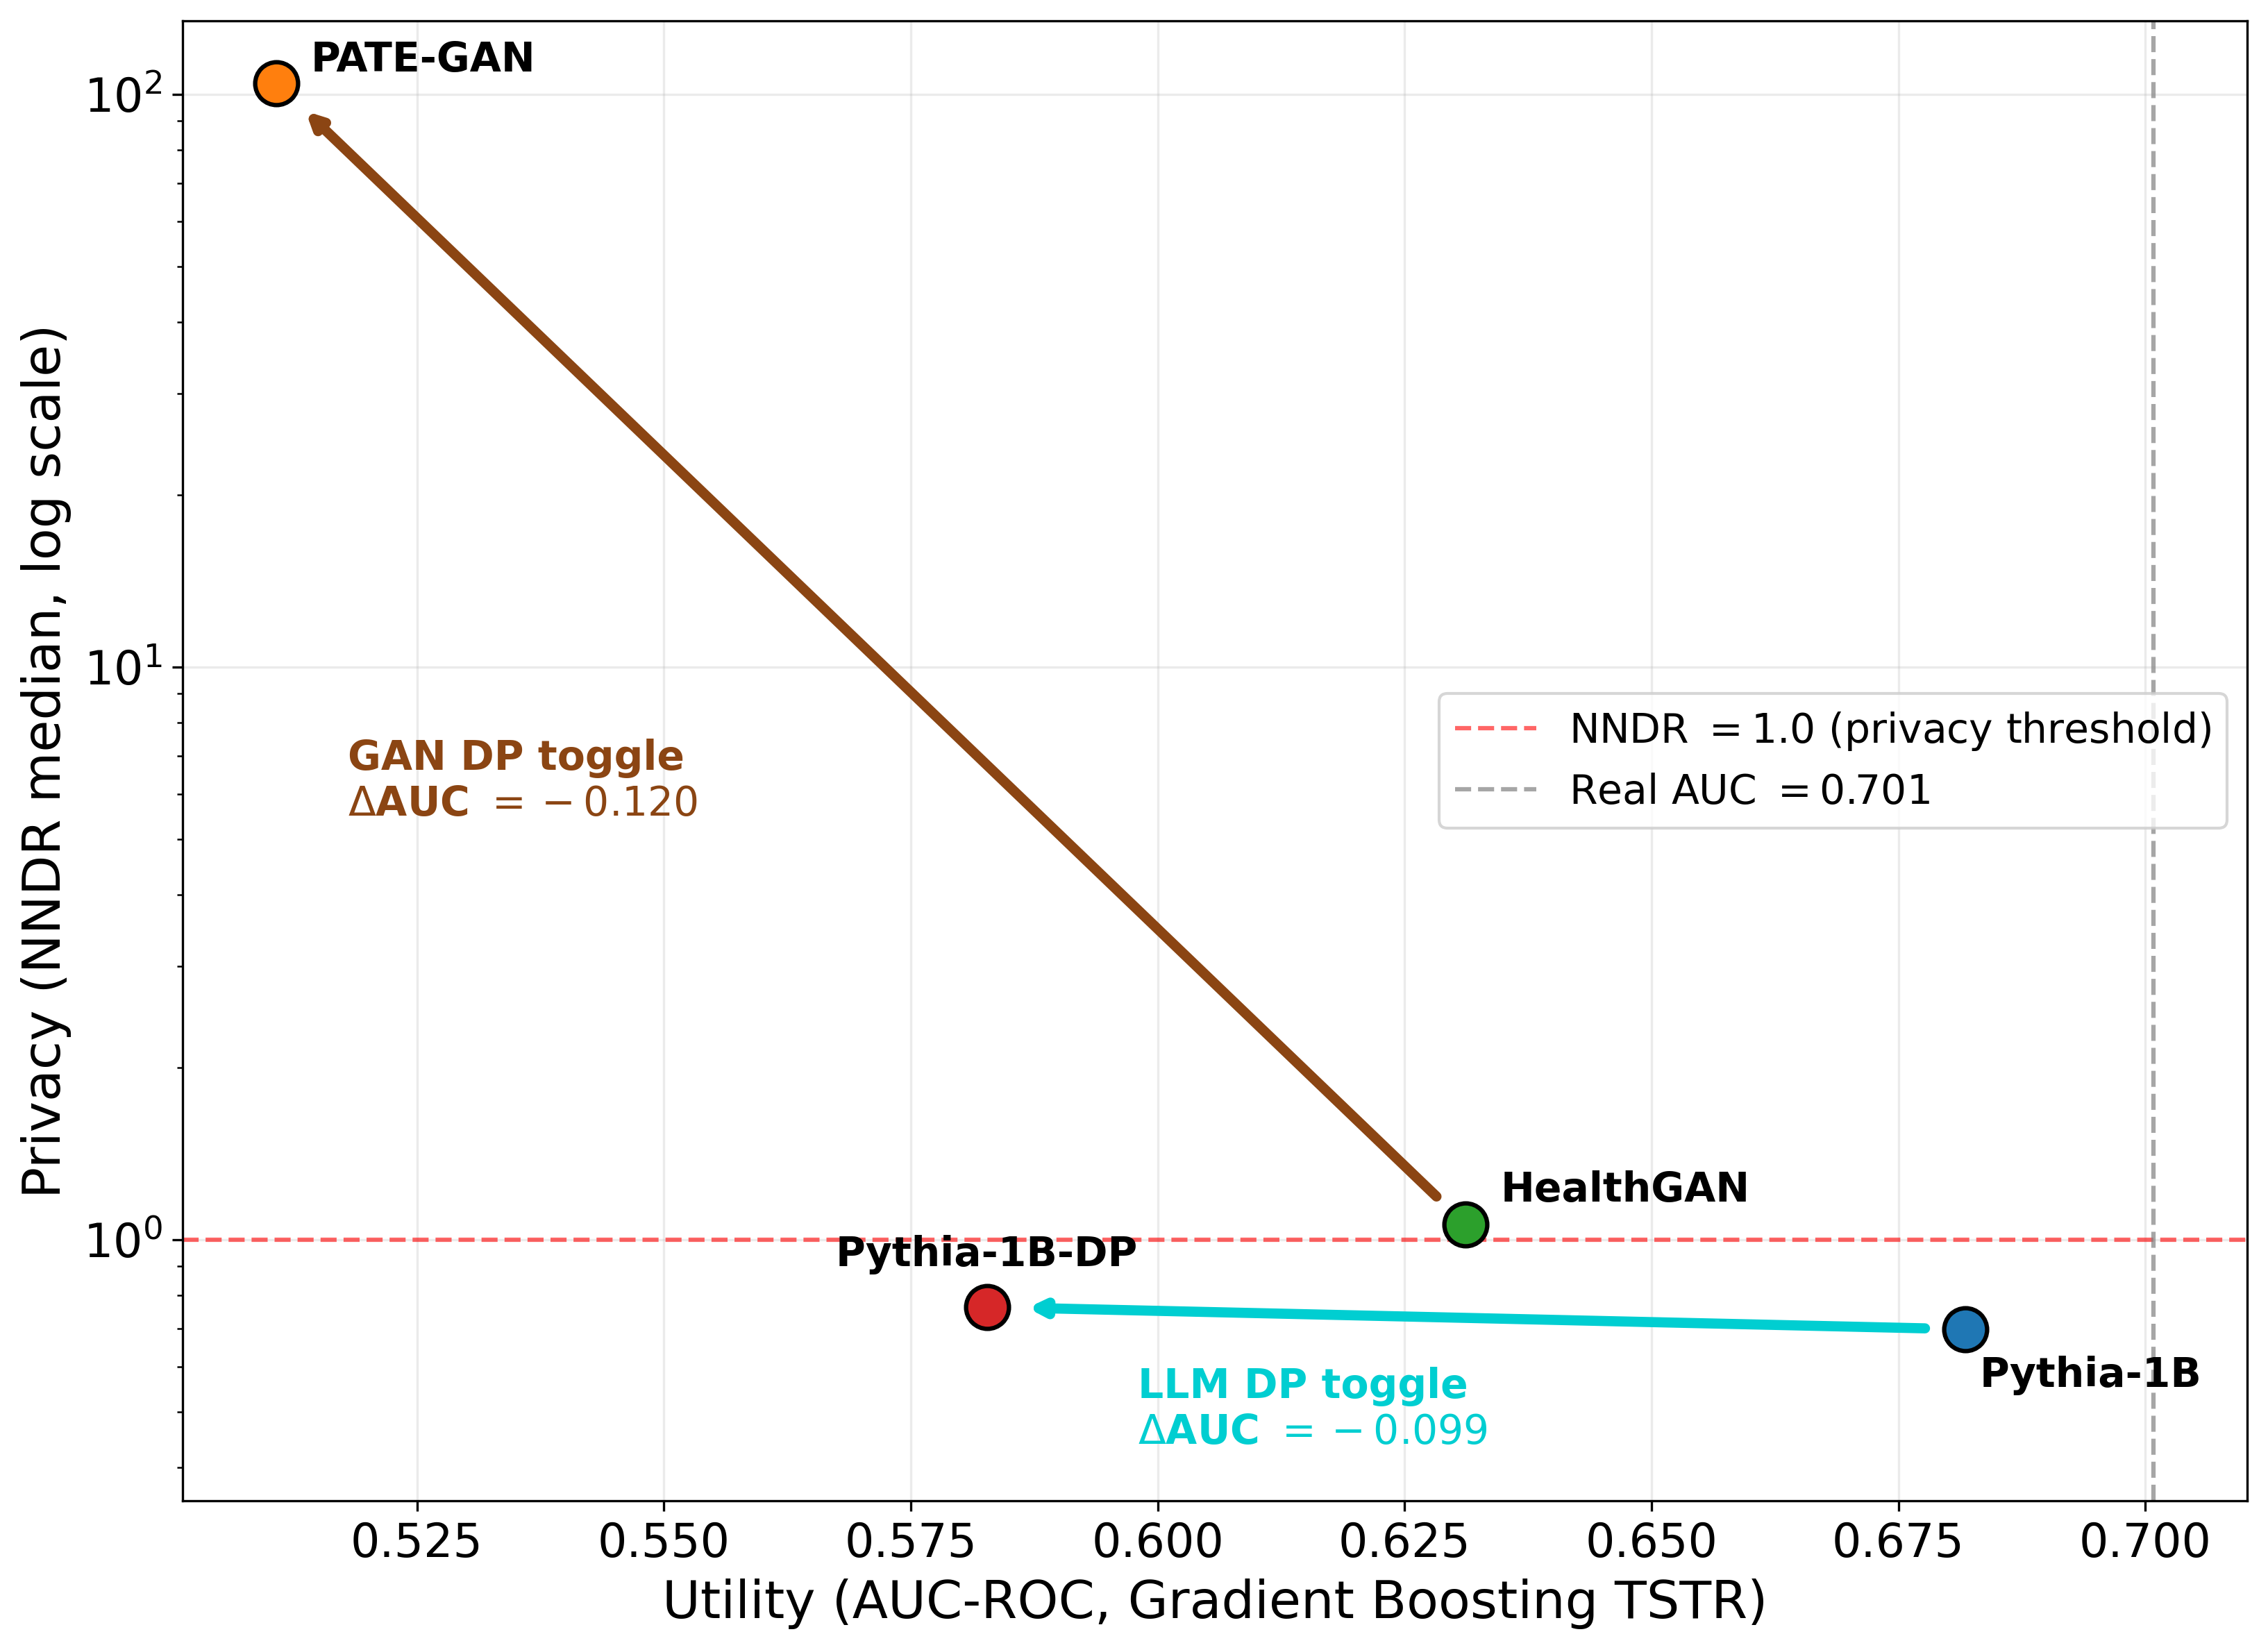
\includegraphics[width=0.82\textwidth]{images/results/arrow}
\caption{Within-family differential-privacy changes on the privacy and
utility plane. The arrows compare HealthGAN with PATE-GAN for the GAN
family and Pythia-1B with Pythia-1B-DP for the LLM family. The vertical
axis uses a logarithmic scale. PATE-GAN's high NNDR reflects its large
distance from the real-data distribution, as discussed in
Section~\ref{sec:results:rq2:privacy}.}
\label{fig:rq3:arrow}
\end{figure}

The two arrows differ sharply in length and meaning. The LLM arrow is
short and almost horizontal. It moves left by $0.0991$ in utility and only
slightly upward in NNDR, a controlled step that keeps the private variant
within the usable region of the plane. The GAN arrow is long and steep,
moving the operating point from HealthGAN's usable position down and to the
left to PATE-GAN's degenerate position. As noted, its vertical extent
reflects the off-manifold distance artefact rather than a genuine privacy
gain. Read together, the figure shows
that the controlled, architecture-matched differential-privacy step (the
LLM arrow) is far less destructive to utility than the GAN-side
transition, and that the only differentially private generator to remain
in the usable region of the plane is the LLM one.

\subsection{Supplementary Per-Family Analyses}
\label{sec:results:rq3:supplementary}

The full per-generator diagnostics underlying both transitions are
referenced rather than re-plotted here. The complete metric values for all
four generators appear in the comprehensive summary of
Table~\ref{tab:rq2:summary}. The per-generator correlation-difference
heatmaps and Cox hazard-ratio plots for HealthGAN, PATE-GAN, Pythia-1B, and
Pythia-1B-DP are collected in Appendix~\ref{app:utility-diag}, where the
two within-family pairs can be compared panel by panel.

\subsection*{Findings for Research Question 3}
\label{sec:results:rq3:answer}

At the same target privacy budget of
$(\varepsilon,\delta)=(5.0,10^{-5})$, the two model families showed
notably different privacy-utility trade-offs. 
The Pythia-1B transition kept statistical fidelity
comparatively well and improved selected empirical privacy diagnostics,
but incurred a substantial reduction in predictive utility. In contrast,
the HealthGAN-to-PATE-GAN transition was associated with a much broader
loss of fidelity and utility. However, because the GAN configurations
also differ in architecture and training procedure, this deterioration
cannot be attributed to differential privacy alone.

Within the LLM family, Pythia-1B-DP had a TSTR AUC-ROC decrease of
$0.0991$ and an F1 decrease of $0.2322$ relative to Pythia-1B. Mean KS
increased by $0.0187$ and pairwise correlation difference increased by
$0.0260$. It indicates smaller losses in marginal and linear-dependency
fidelity than in predictive performance. Cox confidence-interval overlap
remained unchanged at $7/13$.

The LLM-side privacy improvement was selective rather than consistent
across all metrics. For Pythia-1B-DP, the maximum attribute-inference advantage decreased
from $+0.0410$ to $-0.0056$. This result indicates that the evaluated
attack did not outperform the baseline. Outlier linkability also
decreased from $0.6\%$ to zero. Median NNDR moved from $0.698$ to
$0.763$ which is towards the real-to-real spacing reference. In contrast,
membership-inference AUC remained effectively unchanged at approximately
$0.5$, and NNAA privacy loss remained close to zero for both variants.
NNAA test accuracy increased from $0.6204$ to $0.7139$, showing that the
private synthetic data became easier to distinguish from real data.
Differential privacy therefore improved the observed attribute- and
outlier-specific risks, but did not improve every empirical privacy
dimension.

Within the GAN family, HealthGAN to PATE-GAN transition was
associated with substantially larger utility and fidelity losses.
AUC-ROC decreased by $0.1204$, F1 decreased by $0.3731$, mean KS
increased by $0.4901$, and pairwise correlation difference increased by
$0.0806$. Cox confidence-interval overlap also changed from $7/12$ to
$0/13$. PATE-GAN's median NNDR increased from $1.063$ to $104.601$, but
this cannot be interpreted as an empirical privacy improvement. The
extreme distance occurred together with an NNAA test accuracy of $0.9999$
indicates that PATE-GAN generated records
far outside the real-data distribution. Its zero outlier linkability is
therefore uninformative.

Comparing the resulting private configurations, Pythia-1B-DP retained
substantially higher predictive and statistical-similarity utility than
PATE-GAN. It achieved an AUC-ROC of $0.5827$ compared with $0.5108$, an
F1 score of $0.2714$ compared with $0.0093$, a mean KS of $0.0992$
compared with $0.5381$, and a correlation difference of $0.0466$
compared with $0.1142$. Thus Pythia-1B-DP remained within a usable, utility-reduced region
of the privacy-utility profile, whereas PATE-GAN did not at the same privacy budget.

These findings provide stronger evidence about the DP-SGD-associated
change within the LLM family because the Pythia variants share the same
backbone and data representation. The GAN comparison instead combines 
the effects of architecture, training
procedure, and privacy mechanism. Consequently,
the results do not constitute a controlled comparison of DP-SGD and PATE,
nor do they show that one mechanism is generally superior. They show that,
for the evaluated configurations, the LLM-based private model degraded
more gracefully under the matched target privacy budget. The failed
Pythia-70M DP-SGD run further indicates that this result should not be
generalised across LLM scales. All reported differences remain
descriptive point estimates without repeated-run uncertainty and are
limited to the evaluated utility and privacy metrics.

\cleardoublepage
